% This template was originally by R. Jacob Vogelstein
% Updated on March 1, 2010 by Noah J. Cowan


\documentclass[12pt,oneside,final]{thesis}
\usepackage{Sweave}
\usepackage{cite}

\usepackage{amssymb,amsmath,amsthm,amscd}
\usepackage{graphicx}
\usepackage{subcaption}
\graphicspath{{./figs/}}
\usepackage{hyperref, mathrsfs, bm}

\usepackage{url}
\renewcommand{\thesubfigure}{}
% justifying
\usepackage{ragged2e}




\graphicspath{{./}{./../DataFusion/}{./../DataFusion/graphs/}{./../DataFusion-graphmatch/graphs/}{./../VertexCorrespondence/graphs/}}

\usepackage{fixltx2e}
\usepackage{array}
% wrapfig is fragile: use sparingly
\usepackage{wrapfig} 
%\usepackage{times}  % Use this for ugly fonts
\usepackage{verbatim}

\usepackage{fancyhdr}    % Use nice looking headers along with the required footer page numbers   
%\usepackage[hypertex]{hyperref}

%Define the header/footer style
\pagestyle{fancy}
\fancyhf{}
\setlength{\headheight}{15pt}
\lhead{\leftmark}
\cfoot{\thepage}
\renewcommand{\headrulewidth}{0pt}
\fancypagestyle{plain}{% Redefine ``plain'' style for chapter boundaries
\fancyhf{} % clear all header and footer fields
\fancyfoot[C]{\thepage} % except the center
\renewcommand{\headrulewidth}{0pt}
\renewcommand{\footrulewidth}{0pt}}

\newtheorem{thm}{Theorem}
\newtheorem{cor}{Corollary}
\newtheorem{lem}{Lemma}

%\DeclareMathOperator*{\argmin}{arg\,min}

\newcommand{\myred}{\color{red}}
\newcommand{\mygreen}{\color{green!50!black}}
\newcommand{\myblue}{\color{blue}}

\newcommand{\mcX}{\mathcal{X}}
\newcommand{\mcY}{\mathcal{Y}}
\newcommand{\mcG}{\mathcal{G}}
\newcommand{\mcF}{\mathcal{F}}
\newcommand{\argmax}{\ensuremath{\arg\max}}
\newcommand{\argmin}{\ensuremath{\arg\min}}
\newcommand{\logodds}{\ensuremath{\mbox{log odds}}}
\newcommand{\Pos}{\ensuremath{\mbox{Pos}}}
\newcommand{\Neg}{\ensuremath{\mbox{Neg}}}
\newcommand{\Star}{\ensuremath{\mbox{star}}}
\newcommand{\Error}{\ensuremath{\mbox{Error}}}
\newcommand{\diag}{\ensuremath{\mbox{diag}}}
\newcommand{\degrees}{\ensuremath{\mbox{degrees}}}
\newcommand{\1}{\ensuremath{\mbox{{\bf 1}}}}
\newcommand{\Real}{\mathbb{R}}
\newcommand{\iid}{\stackrel{iid}{\sim}}


\newcommand{\mA}{\mathcal{A}}
\newcommand{\mD}{\mathcal{D}}
\newcommand{\mK}{\mathcal{K}}
\newcommand{\mC}{\mathcal{C}}
\newcommand{\mM}{\mathcal{M}}
\newcommand{\mN}{\mathcal{N}}
\newcommand{\mT}{\mathcal{T}}
\newcommand{\mI}{\mathcal{I}}
\newcommand{\mX}{\mathcal{X}}
\newcommand{\mY}{\mathcal{Y}}
\newcommand{\mZ}{\mathcal{Z}}
\newcommand{\mF}{\mathcal{F}}
\newcommand{\mP}{\mathcal{P}}


\newenvironment{remark}[1][Remark]{\begin{trivlist}
\item[\hskip \labelsep {\bfseries #1}]}{\end{trivlist}}



%\tolerance=10000

%\makeglossary % enable the glossary

\begin{document}
\input{thesis-concordance}

\title{JHU THESIS TEMPLATE}
\author{Sancar Adali}
\degreemonth{May}
\degreeyear{2013} 
\dissertation
\doctorphilosophy
\copyrightnotice


% add your chapters, best way is to have separate TeX files for each chapter

%% FRONTMATTER
\begin{frontmatter}

% generate title
\maketitle

\begin{abstract}

Abstract goes here.

\vspace{1cm}

\noindent Primary Reader: Carey E Priebe\\
Secondary Reader: Daniel E Fishkind

\end{abstract}

\begin{acknowledgment}

Thanks!

\end{acknowledgment}

\begin{dedication}
 
This thesis is dedicated to \ldots

\end{dedication}

% generate table of contents
\tableofcontents

% generate list of tables
\listoftables

% generate list of figures
\listoffigures

\end{frontmatter}
\chapter{Introduction}
\label{sec:intro}
\chaptermark{Optional running chapter heading}


Different views of the data

\section{Data Settings}


 It is a challenge  to do a tractable analysis on data from disparate sources of data (such as multiple sensors). The multitude  of sensors technology and large numbers of sensors both are  sources of difficulty and hold promise for efficient inference.
 The typical multiple sensor setting is visualized in  Figure ~\ref{fig:fig1}.

\begin{figure}
\centering
\includegraphics[scale=0.75]{gen-model-orig-proj.pdf}
\caption{Multiple Sensor setting}
\label{fig:fig1}
\end{figure}

It is assumed some objects lie in some "object`` space $\Xi$, and each sensor has another "view`` of the objects. The measurements recorded by the $i^{th}$ sensor lie in some "measurement space`` $\Xi_i$. The usual approach in pattern recognition is to use feature extractors on the spaces to get a feature representation in Euclidean space and use classical pattern recognition tools to carry out the exploitation task. The alternative approach is to acquire dissimilarities between the group of objects, and use the dissimilarities to either find an embedding in a low-dimensional Euclidean space where classic statistical tools are available for inference or use dissimilarity-based versions of pattern recognition tools~\cite{duin2005dissimilarity}. The embedding approach in a  low-dimensional Euclidean space will be used where the small number of embedding dimension allow us to avoid "curse of dimensionality``. Also, the embeddings of dissimilarities from  different conditions will be required to be "commensurate`` so that sensor measurements can be compared or jointly used in inference. This is accomplished by maps $\rho_k,k=1,\ldots,K$ from measurement spaces $\Xi_k$ to a low-dimensional commensurate space $\mathcal{X}$ visualized in~\ref{fig:fig1}. Learning these maps from data is  an important portion of the proposed  approach.


\label{sec:data}


\section{Dissimilarity representation}
 Great progress been made in the theory and applications of pattern recognition, particularly in problem settings where the data available or assumed to be available as vectors in metric spaces. There are still many problems where due to the nature of setting, one only has access to dissimilarities or  proximities or distances between measurements or subjective assessment  of similarities of objects. We thus have a superficial distinction between these two kinds of settings, even though the inference task doesn't distinguish between this representation issue. The gap between the two kinds of representation of data can be bridged using various  techniques, such as different kinds of embedding and computing appropriate distances .
We will refer to the entities of interest for pattern recognition as objects. These might be real objects or abstract concepts. The data will be a collection of measurements for instances or examples of these objects.
 \cite{Duin} is a book that compiles the fruits of research in learning from  dissimilarity-based representation. In the introduction, the authors make clear the distinction between statistical and structural(syntactic) pattern recognition, which is previously discussed in \cite{NadlerSmith1993}. The first is concerned with the analysis of features which are lists of measured values for object attributes. The second uses a relational view of objects for representation. In both cases,  the task of discrimination  can rely on distances (however they are defined). Pekalska and Duin  suggest dissimilarity measures  are a natural bridge between the two types of information and this applicability to  multiple settings is one of the motivating factors for our use of dissimilarity representation in information fusion. 
For feature-based representation, one first defines the features which are either raw or processed measurements from sensors observing the objects and  represention of each object is a single point in the representation space. Dissimilarity-based representation relies on a dissimilarity measure, a way of quantifying the dissimilarity, proximity or similarity between any two objects. It is quite possible, in fact preferable, that the dissimilarity is \emph{designed for} the inference task at hand. 
%\cite{Duin} argue this is a reason dissimilarities can be superior, since similarities can encode concepts of class membership directly in class discrimination problems.
There are naturally multiple ways (some more natural than others) of comparing entities and this fact will provide one of the arguments for our approach to information fusion from  data sources, even sources that collect  data of same modality. In  the latter case where the data comes from separate sources but of the same type, the same measurements might have different dissimilarity representation according to subjective judgments or different dissimilarity  measures. 

\section{Matched Measurements}
Data fusion is a very general concept and the specific setting of data fusion should be clarified here. The exploitation task we are interested in might involve (perhaps notional) complex objects or abstract entities that are not practically representable. The objects are members of a (perhaps notional) space called "object`` space, $\Xi$ in Figure \ref{gen-model} . We will have different "views``, "measurements`` or "data modalities`` extracted from these objects (which we will refer to as "conditions"), and these observations will be members of the measurement space for those "conditions" ($\Xi_k$ for $k^{th}$ condition). Each example of the objects will have an observation in each of the different conditions and the corresponding observations across different "conditions`` will be "matched``.Given new observations from these different "conditions``, is it possible to decide if they are "matched``? Or if a group of  observations from each condition are "matched`` to each other, but the specific correspondences are unknown, is it possible to find the true correspondences? Different approaches are proposed in this dissertation to address these questions.

For $n$ different objects, each of the measurements $x_{ik}$ lies in  the corresponding space $\Xi_k$ and the  measurements $x_{ik}$ are matched for the same $k$ index
\[  \begin{array}{cccc}
        & \Xi_1 & \cdots & \Xi_K\\
        Object ~ 1 & \bm{x}_{11} & \sim \cdots \sim & \bm{x}_{1K} \\
        \vdots & \vdots & \vdots & \vdots \\
        %\text{Object} ~ i & \bm{x}_{i1} & \sim \cdots \sim & \bm{x}_{iK} \\
        %\vdots & \vdots & \vdots & \vdots \\
        Object ~ n & \bm{x}_{n1} & \sim \cdots \sim & \bm{x}_{nK}
      \end{array}      
\]
To each pair of measurements $x_{ik},x_{jk}$ in the same space, we can assign a dissimilarity value $\delta_{ijk}=\delta\{x_{ik},x_{jk}\}$, possibly dependent on the space $\Xi_k$. We assume the dissimilarities to be non-negative and  symmetric, and 0 for $\delta\{x_{ik},x_{ik}\}$  It is this training set of  dissimilarities we utilize to do inference on the following exploitation task:

 Given dissimilarities between  $K$ new measurements/observations ($\bm{y}_{k};k=1,\ldots,K$) and the previous 
$n$ objects under $K$ conditions,    test the null hypothesis  that ``these measurements are from the same  object"  against the alternative hypothesis that ``they are not  from the same  object"~\cite{JOFC}:
    \[
\begin{array}{l}
%\hspace{-2em}
    H_0: \bm{y}_{1} \sim \bm{y}_{2} \sim \cdots \sim \bm{y}_{K}
 \text{ versus } 
 H_A: \exists i, j , 1\leq i < j \leq K :\bm{y}_{i} \nsim \bm{y}_{j}  
\end{array}
\]
 The null hypothesis can be restated as the case where the dissimilarities are ``matched" and the alternative as the case where they are not ``matched".

Dissimilarities are in the form  of $n \times n$  dissimilarity matrices $\{\Delta_k;k=1,\ldots,K\}$ with entries $\{\delta_{ijk} ;  i=1,\ldots,n;\hspace{5pt} j=1,\ldots,n\}$  and a  vector (of length $nK$) of dissimilarities  $\mathbf{\Delta}^{new}=\{ \delta_{ik}^{new}; i=1,\ldots, n;\hspace{5pt} k=1,\ldots,K\}  $  where $\delta_{ik}^{new} $ is the dissimilarity  between  $x_{ik}$ and $y_k$

 Since dissimilarities are  measured between pairs of objects under the same condition, they will be the entries in  
 separate dissimilarity matrices , each matrix consisting of dissimilarities between pairs of  measurements for a separate condition.
 

 
 
The inference task  is to find a collection of mappings (one from each "condition``) to a lower dimensional space where new observations from each condition can be mapped to be made commensurate. These mappings does not need to be explicitly defined; they can be a collection of embedding routines. As long as the embedding of the dissimilarity results in a  the mapping is unique,  out-of-sample embeddings could be added to the embedding of in-sample dissimilarities.

A few points should be mentioned to distinguish our approach from related approaches.
 Due to the fact that data sources are ``disparate", it is not immediately obvious how  a dissimilarity between an object in one condition and another object in another condition  can be computed, or even defined.  In general, these between-condition between-object  similarities are not available.
 
 Whether these observations are , by default,  in dissimilarity representation for each condition, or dissimilarities are computed for the observations which are feature observations at each condition is not relevant to our exploitation task: it is assumed one way or another (perhaps from experts in the domain of the problem),  dissimilarities for each condition are available for inference purposes. 

The exploitation task  being considered is \emph{not} accurate reconstruction of these feature observations, even if they do exist. The quality of the  embeddings need only to be  good enough to be useful in the inference task. Therefore, the quality of our representation will be dependent on the bias-variance tradeoff, where by choosing a low-dimensional representation, we might be introducing more model bias, but the representation will be more stable and robust with respect to noise.
\chapter{Related work}
\label{sec:Related}
\chaptermark{Optional running chapter heading}



\section{Multiple View Learning}
\label{sec:section}



\section[Domain Adaptation]{Transfer Learning}


\section[Manifold Matching]{Manifold Alignment}
There have many efforts toward solving ``manifold alignment", which is a related  problem. ``Manifold alignment" seeks to find correspondences between observations from different ``conditions". The setting that is most similar to ours is the semi-supervised setting, where a set of correspondences are given and the task is to find correspondences between a new set of points in each condition. In contrast, our hypothesis testing task is to determine whether any given pair of points is ``matched" or not. The proposed solutions follow a common approach in that they look for a common commensurate or a latent space, such that the representations (possibly projections or embeddings) of the observations in the commensurate space match.

Wang and Mahedavan~\cite{Wang2008} suggest an  approach that uses embedding followed by Procrustes Analysis to find a map to a commensurate space. Given a paired set of points, Procrustes Analysis~\cite{Sibson}, finds a transformation from one set of points to another in the same space that minimizes sum of squared distances, subject to some constraints on the transformation. In the case mentioned in \cite{Wang2008}, the paired set of points are corresponding low-dimensional embeddings of kernel matrices.   For the embedding step, they made the choice of using Laplacian Eigenmaps, though their algorithm allows for any appropriate embedding method.

 Zhai et al.~\cite{Zhai2010}  finds two projection matrices to minimize three terms in an energy function similar to our JOFC approach (see Section \ref{sec:JOFC}). One of the terms is the \emph{correspondence preserving term} which is the sum of the squared distances between corresponding points and is analogous to our commensurability error term. The other two terms are \emph{manifold regularization terms} and consist of the reconstruction error for a Locally Linear Embedding of the projected points. These terms, analogous to fidelity, make sure the projections in the lower dimension retain the structure of the original points. For fidelity error terms in our setting, this is done by preserving dissimilarities. For manifold regularization terms, this is done by preserving the local neighborhood of points, such that close points are not mapped apart.
Ham and Lee solve the problem in semi-supervised setting by a similar approach, by minimizing a cost function of three terms, two terms for fidelity of embedding, one term of commensurability.


Another view to look at the data from different sources is to consider disparate data as different views to be reconciled. According to this view, for observations of $n$ objects under $K$ conditions, $n$ points are embedded instead of $nK$ points. Choi et al.\ \cite{Choi:2008:MIM:1619995.1620064} use the Markov random walk interpretation of multiple kernel matrices to combine into one kernel matrix.  Many other ``Multiple Kernel Learning"  methods exist in the literature~\cite{McFee:2011:LMS:1953048.1953063,Lin2009,Lanckriet2004}.

Another approach is Three-way Multidimensional scaling\cite{3wayNMDS,borg+groenen:1997}.
 This approach assumes the  different ``conditions" of the data are linear transformations of a single configuration and aims to find this single configuration. For our setting, one would first embed the in-sample dissimilarities via the three-way MDS, which would give as the linear transformations that map from group configuration to individual configurations under each condition. This is followed by out-of-embedding the OOS dissimilarities, and use the inverse of the transformation matrices to find the out-of-sample embeddings with respect to the group configuration. Since the out-of-sample embeddings are commensurate, the test statistic can be computed as the distance between the OOS embeddings. 
\chapter{Multidimensional Scaling and Its Variants}
\label{sec:MDS}
\chaptermark{Optional running chapter heading}

Introduction to MDS and dissimilarity representation to MDS

\section{Multidimensional Scaling in the general setting}
Multidimensional Scaling is  a method to  (MDS)~\cite{CMDS,borg+groenen:1997,duin2005dissimilarity}  embed dissimilarities between examples  in the Euclidean space  with a chosen dimension $d$ such that the distances between the embeddings are as close as possible (in various senses) to the original dissimilarities. Different criterion functions can be used to measure how close the distances are  to the given dissimilarities, leading to different embedded configurations. These different variants of MDS can be described using a single formulation.
\label{sec:section}
Consider a  set of n objects. For each pair of objects, the dissimilarity value, denoted by $d_{ij}$ is a non-negative real number which quantifies how dissimilar those two objects are. The collection of these values form the matrix $\Delta$ , which is  a $nxn$ dissimilarity matrix. While ,generally, dissimilarities between finite set of objects are being considered; for a dissimilarity matrix, we can consider the objects as points in a space, whose neighborhood relationship is defined by the dissimilarity measure  . The dissimilarities have to satisfy $\delta_{ij}\geq 0$ and $\delta_{ii}=0$ and $d_{ij}=d_{ij}$. Therefore  $\Delta$ is non-negative, hollow and symmetric. If, in addition, each triplet of dissimilarities $\delta_{ij}$, $\delta_{ik}$ and $\delta_{ik}$  satisfy the triangle inequality, then D is called  an Euclidean distance matrix.

\section{Different criterion for MDS?}
Multidimensional Scaling finds a configuration of points consistent with given dissimilarities in a finite dimensional Euclidean space. There are various variants of MDS that use different measure of consistency.  In general, the criteria minimize discrepancy between $f(\delta_ij)$ and  $d(\bm{x_i},\bm{x_j})$ where d is the Euclidean distance function and $f(\cdot)$ is monotonically increasing function. Depending on whether ``metric" or ``non-metric" MDS is being considered, $f(\cdot)$ is either a linear transformation or a non-linear one.


\subsection{Metric MDS}
 For metric MDS, transformations of the form  $f(x)=ax+b$ are allowed.
 \subsubsection{Stress Criterion}
 Setting $f(x)=x$ and choosing  the discrepancy measure between the dissimilarities and distances of embedded points to be $\ell_2$, the resulting criterion is called the raw stress criterion. Additionally weights($w_{st}$) can be introduced for each discrepancy term. Denote the matrix composed of the weight by $W$.
 \begin{equation}
\sigma_{W}(X)=\sum_{1\leq s\leq n;1\leq t\leq n} {w_{st}(d_{st}(X)-\delta_{st})^2  }\label{raw-stress}
\end{equation}
Subtypes of Stress criterion is identified by different choices for $w_st$ which depend on the original dissimilarities $\delta_{st}$ .
For example, choosing $w_{st}={\sum{\delta_{st}^2}}^{-1}$ normalizes the stress so that the stress value is always between 0 and 1. One can compare different configurations by this standardized stress value and conclude whether a configuration is a good fit or not based on this value.
A slightly different weighting scheme is $w_{st}=\{ \sum_{st}{\delta_{st}-\bar{\delta} } \}^{-1}$ 
where $\bar{\delta}=\frac{1}{(n)(n-1)} \sum{\delta_{st}}$ (average of dissimilarities). 
Another related criterion is SSTRESS criterion which involves squares of dissimilarities and distances:
\[
=\sum_{1\leq s\leq n;1\leq t\leq n} {(d_{st}^2(X)-\delta_{st}^2)^2  }
\]


\subsubsection{Sammon Mapping Criterion}
This is a specific case of the Stress criterion where the weights $w_{st}$ are set to be $\delta_{st}^{-1} \{\sum_{k<l}\delta_{kl} \}^{-1}$. These set of weights normalizes the squared discrepancies in the stress criterion by the magnitude of the original dissimilarities, so that discrepancy terms for the larger dissimilarities do not dominate the optimization of the criterion function. As a result, small $\delta_{st}$ are preserved.

\subsection{Ordinal (Nonmetric) MDS}
 For Nonmetric MDS, $f(\cdot)$    is allowed to be  any monotonic transformation. Specifically in psychometric applications of MDS, the assumption that the dissimilarities are a scaled-shifted version of the ``true"  dissimilarity is an unwarranted assumption. It is possible the existence of a ``true" dissimilarity is in question. Even if the dissimilarities are physical distances, humans tend to have biased estimates of those distances (long distances are usually underestimated ). \cite{Trosset1998}. This variant of MDS is also called ordinal, because what is preserved is the rank of dissimilarities, not their magnitude.

\section{Classical MDS and the Strain Criterion}

Consider the case where $\Delta$ is Euclidean. So there exist $\bm{x}_{i}$ such that $\forall \quad s,t$ $\bm{x}_{s}$ and $\bm{x}_{t}$ such that $\delta_{st}=d(\bm{x}_{s}-\bm{x}_{t})$. If $\bm{x}_{i}$ satisfy $\delta_{st}=d(\bm{x}_{s}-\bm{x}_{t})$,  $\bm{x}_{i}+\bm{u}$ for a constant vector $\bm{u}$. To remove this ambiguity   $\sum{\bm{x}_{i}}$ is set to $\bm{0}$.
\[
\delta_{st}^2= d(\bm{x}_{s},\bm{x}_{t})^2 = \|\bm{x}_{s}   \|^2 +   \|\bm{x}_{t}   \|^2   -   2  \bm{x}_{s} \cdot  \bm{x}_{t}   
\]
Reorganizing terms,
\begin{align}
-\frac{1}{2} \{ \delta_{st}^2 +\|\bm{x}_{s}   \|^2 +\| \bm{x}_{t} \|^2 \}   = \bm{x}_{s}   \cdot\bm{x}_{t}
\label{delta_{st}}
\end{align}
Summing over $s$, over $t$ and then over $s$ and $t$, we get the following identities

\begin{align*}
\sum_s{ \delta_{st}^2} &= \sum_s{\| \bm{x}_{s}   \|^2} + n \|\bm{x}_{t}   \|^2 -2 \sum_s{ \bm{x}_{s}   \cdot\bm{x}_{t}    } \quad s=1,\ldots,n\\
\sum_t{ \delta_{st}^2} &= \sum_t{\| \bm{x}_{t}   \|^2} + n\|\bm{x}_{s}   \|^2  -2 \sum_t{ \bm{x}_{s}   \cdot\bm{x}_{t}   } \quad t=1,\ldots,n \\
\sum_{st}{ \delta_{st}^2} &= 2n\sum_{t}{\| \bm{x}_{t}   \|^2}  -2\sum_{s}{ \bm{x}_{s} } \cdot \sum_t{   \bm{x}_{t} }\\
\end{align*}

Dividing each equality by $\frac{1}{n}$ , $\frac{1}{n}$ and $\frac{1}{n^2}$ respectively and using the fact that $\sum{\bm{x}_{i}}=\bm{0}$

\begin{align*}
\frac{1}{n}\sum_s{ \delta_{st}^2} &= \frac{1}{n}\sum_s{\|\bm{x}_{s}   \|^2 } +  \|\bm{x}_{t}   \|^2 \quad   t=1,\ldots,n\\
\frac{1}{n}\sum_t{ \delta_{st}^2} &= \frac{1}{n}\sum_t{\|\bm{x}_{t}   \|^2 }+  \|\bm{x}_{s}   \|^2 \quad   s=1,\ldots,n\\
\frac{1}{n^2}\sum_{st}{ \delta_{st}^2} &= \frac{2}{n}\sum_{t}{\|\bm{x}_{t}   \|^2} \\
\end{align*}

Reorganizing terms,
\begin{align*}
\|\bm{x}_{t}   \|^2  &= \frac{1}{n}\sum_s{ \delta_{st}^2} + \frac{1}{n}\sum_s{\|\bm{x}_{s}   \|^2   } \\
\|\bm{x}_{s}   \|^2  &= \frac{1}{n}\sum_t{ \delta_{st}^2} + \frac{1}{n}\sum_t{\|\bm{x}_{t}   \|^2  }\\
0 &= -\frac{2}{n}\sum_{t}{\|\bm{x}_{t}   \|^2} +\frac{1}{n^2}\sum_{st}{ \delta_{st}^2} \\
\end{align*}


Summing the three equations and replacing with  $\|\bm{x}_{s}   \|^2 +\|\bm{x}_{t}\|^2$ in original equation

\[
\delta_{st}^2= \frac{1}{n}\sum_s{ \delta_{st}^2} + \frac{1}{n}\sum_s{\|\bm{x}_{s}}   \|^2 + \frac{1}{n}\sum_t{ \delta_{st}^2} + \frac{1}{n}\sum_t{\|\bm{x}_{t}}  \|^2  -\frac{2}{n}\sum_{t}{\|\bm{x}_{t}   \|^2} +\frac{1}{n^2}\sum_{st}{ \delta_{st}^2}   -2\bm{x}_{s}   \bm{x}_{t}   \|
\]

\[
\delta_{st}^2= \frac{1}{n}\sum_s{ \delta_{st}^2} +  \frac{1}{n}\sum_t{ \delta_{st}^2}  +\frac{1}{n^2}\sum_{st}{ \delta_{st}^2}  -2\bm{x}_{s}   \bm{x}_{t}   \|
\]


\[
\bm{x}_{s}   \bm{x}_{t} = \frac{-1}{2} \{\delta_{st}^2 - \frac{1}{n}\sum_s{ \delta_{st}^2} -  \frac{1}{n}\sum_t{ \delta_{st}^2}  +\frac{1}{n^2}\sum_{st}{ \delta_{st}^2 }     \| \}
\]







Some of the sums in the above expression can be written in matrix notation,
\begin{align*}
\bm{1}^{T}\Delta^2= \frac{1}{n}\sum_s{ \delta_{st}^2}
\Delta^2 \bm{1} = \frac{1}{n}\sum_t{ \delta_{st}^2}
\end{align*}
So 
\begin{align*}
XX^T = \frac{-1}{2} \{\Delta^2 -  \frac{1}{n} \bm{1}\bm{1}^{T}\Delta^2  -  \frac{1}{n} \Delta^2 \bm{1}\bm{1}^{T} +   \frac{1}{n^2} \bm{1}\bm{1}^{T}\Delta^2 \bm{1}\bm{1}^{T}      \}
\end{align*}





\section{Effect of Noise}

\section{Maximum Likelihood MDS and MULTISCALE}
\section{3-way MDS}

\section{Optimization Issues: Local Minima}
\chapter{Fidelity and Commensurability}
\label{sec:FidComm}
\chaptermark{Optional running chapter heading}

The concepts of  Fidelity and Commensurability
Unless 
\begin{itemize}
\item the dissimilarity matrix is the Euclidean distance matrix of the original observations, and, 
\item the embedding dimension is greater or equal to the dimension of the original observations,
\end{itemize}
MDS with raw stress will not result in a perfect reconstruction  of the original observations. Note that the objective of the embedding is not \emph{perfect} reconstruction, but the best embedding for the exploitation task which is to test whether two sets of dissimilarities are ``matched". What is considered a good ``commensurate" representation will be dependent on how well the information in original dissimilarities that is relevant to the the match detection task is preserved. The following two criteria  embody the two kind of information  that is relevant to this task.


\begin{itemize}
\item Fidelity is how well the mapping to commensurate space preserves the original dissimilarities. The loss of \em{fidelity} can be measured with  within-condition {\em fidelity error} is given by
    \[
\epsilon_{f_{k}} = \frac{1}{{{n}\choose{2}}} \sum_{1 \leq i < j \leq n} (d(\widetilde{\bm{x}}_{ik},\widetilde{\bm{x}}_{jk})-\delta_k(\bm{x}_{ik},\bm{x}_{jk}))^2
\] 
where ${\bm{x}}_{ik}$ is the original observation of the $i^{th}$ object for the $k^{th}$  condition and $\widetilde{\bm{x}}_{ik}$ is the embedded configuration of the $i^{th}$ object  for the $k^{th}$ condition;  $d(\cdot,\cdot)$ is the Euclidean distance function (for the embedding space) and $\delta_k(\cdot,\cdot)$ is the dissimilarity function defined for objects in the $k^{th}$ condition.

\item Commensurability is how well the mapping to commensurate space preserves matchedness of matched observations. The loss of commensurability can be measured by the between-condition {\em commensurability error} is given by
    \[
\epsilon_{c_{k_1k_2}} = \frac{1}{n} \sum_{1 \leq i \leq n;k_1 <k_2} (d(\widetilde{\bm{x}}_{ik_1},\widetilde{\bm{x}}_{ik_2})-{ \delta_{k_1k_2}}(\bm{x}_{ik_1},\bm{x}_{ik_2}))^2
\label{comm-error}
\]
 for conditions $k_1$ and $k_2$; $\delta_{{k_1}{k_2}}(\cdot,\cdot)$ is the (notional) dissimilarity function between measurements in  $k_1^{th}$ and $k_2^{th}$ conditions. Note that ,in general, there are $K$  within-condition fidelity error terms and $\frac{K \times (K-1)}{2}$  between-condition commensurability error terms.

Although  the between-condition dissimilarities of the same object, ${ \delta_{k_1k_2}(\bm{x}_{ik_1},\bm{x}_{ik_2}})$, are not available,  it is not unreasonable in this setting  to set ${ \delta_{k_1k_2}}(\bm{x}_{ik_1},\bm{x}_{ik_2}) = 0$ for all $i,k_1,k_2$.  So diagonal  entries of $L$ in  equation \eqref{omnibus} are  chosen to be all zeroes. Setting these diagonal entries to zero forces matched points to be embedded close to each other. (It is possible that this choice for between-condition dissimilarities might not be optimal. This issue will be ignored in order to focus on the main problem.)

Then, the commensurability error  term becomes
  \[
\epsilon_{c_{k_1k_2}} = \frac{1}{n} \sum_{1 \leq i \leq n;k_1< k_2} (d(\widetilde{\bm{x}}_{ik_1},\widetilde{\bm{x}}_{ik_2})))^2
\]
\end{itemize}

 There is also between-condition {\em separability error} given by
    $$\epsilon_{s_{k_1k_2}} = \frac{1}{{{n}\choose{2}}} \sum_{1 \leq i < j \leq n;k_1 <k_2} (d(\widetilde{\bm{x}}_{ik_1},\widetilde{\bm{x}}_{jk_2})-{ \delta_{k_1k_2}}(\bm{x}_{ik_1},\bm{x}_{jk_2}))^2.$$ This error will be ignored herein, due to the fact that 
$\delta_{k_1k_2}(\bm{x}_{ik_1},\bm{x}_{jk_2})$ is not  available. Although it is possible to impute these dissimilarities, the optimal  imputation is an open question and ignoring these terms provides for investigation of simpler, still open questions.


Note that the omnibus embedding approach tries to jointly optimize fidelity and commensurability , by minimization of some measure of discrepancy between the given dissimilarities (all of which are between-condition or within-condition dissimilarities) and the distances of the embedded configuration. This is most obvious in the  raw stress version of  MDS, since the individual terms can be separated according to whether they are contributing to  fidelity or  commensurability  error.

 Consider the weighted raw stress criterion $\sigma_{W}(\cdot)$ with a weighting matrix $W$, given in equation~\eqref{raw-stress}.
 The omnibus matrix $M$  is a partitioned matrix consisting of matrices from different conditions ($k={1,2}$),  the entries of the matrix will be indexed by 4-tuple ${i,j,k_1,k_2}$ which refers to the entry in the $i^{th}$ row and $j^{th}$ column of the submatrix in  the $k_1^{th}$  row partition and   $k_2^{th}$ column partition. For example, the entry ${M}_{2n,n}$ will have the indices $\{i,j,k_1,k_2\}=\{n,n,2,1\}$ in the new indexing scheme. $D(\cdot)$ and $W$, which are the same size as $M$, follow the same 4-tuple indexing. Then,
 
\begin{align}
\sigma_W(\cdot)  &= & &\sum_{i,j,k_1,k_2} {w_{ij{k_1}{k_2}}(d_{ij{k_1}{k_2}}(\cdot)-M_{ijk_1k_2})^2 } \notag\\
\hspace{3pt} &=& &\underbrace{\sum_{i=j,k_1<k_2}  {w_{ij{k_1}{k_2}}(d_{ij{k_1}{k_2}}(\cdot)-M_{ijk_1k_2})^2}}_{Commensurability}  \hspace{10pt}  &  + &\hspace{2.5em} \underbrace{\sum_{i<j,k_1=k_2}  {w_{ij{k_1}{k_2}}(d_{ij{k_1}{k_2}}(\cdot)-M_{ijk_1k_2})^2  }  } _{Fidelity}\notag\\
\hspace{3pt}&+&  &\underbrace{\sum_{i< j,k_1<k_2}  {w_{ij{k_1}{k_2}}(d_{ij{k_1}{k_2}}(\cdot)-M_{ijk_1k_2})^2  }  } _{Separability}\label{eq:FidCommSep}\hspace{10pt} .
\end{align}


\begin{comment}
\begin{eqnarray}{ccc}
\sigma_W(\cdot)\hspace{3pt}   &= &\sum_{i,j,k_1,k_2} {w_{ij{k_1}{k_2}}(d_{ij{k_1}{k_2}}(\cdot)-M_{ijk_1k_2})^2 } \notag\\
\hspace{3pt} &= &\underbrace{\sum_{i=j,k_1\neq k_2}  {w_{ij{k_1}{k_2}}(d_{ij{k_1}{k_2}}(\cdot)-M_{ijk_1k_2})^2}}_{Commensurability}  \hspace{10pt}  &  + & \underbrace{\sum_{i\neq j,k_1=k_2}  {w_{ij{k_1}{k_2}}(d_{ij{k_1}{k_2}}(\cdot)-M_{ijk_1k_2})^2  }  } _{Fidelity}\notag\\
\hspace{3pt}&+ &\underbrace{\sum_{i\neq j,k_1\neq k_2}  {w_{ij{k_1}{k_2}}(d_{ij{k_1}{k_2}}(\cdot)-M_{ijk_1k_2})^2  }  } _{Separability}\label{eq:FidCommSep2}\hspace{10pt} .
\end{eqnarray}
\end{comment}


Since ${ \delta_{k_1k_2}}(\bm{x}_{ik_1},\bm{x}_{ik_2}) $ are set to 0, the corresponding entries of $M$ in the commensurability terms will be 0.

Since    the separability error is ignored,  the weights for separability terms are chosen to be 0. This also means off-diagonal elements of $L$ in equation \eqref{omnibus} can be ignored. When separability terms are removed from equation \eqref{eq:FidCommSep}, the resulting equation  is a sum of fidelity and commensurability error terms:


\begin{align}
\sigma_W(\cdot)\hspace{3pt}   
\hspace{3pt}&=&\underbrace{\sum_{i=j,k_1< k_2}  {w_{ij{k_1}{k_2}}(d_{ij{k_1}{k_2}}(\cdot))^2}}_{Commensurability}  \hspace{10pt}  &  +&\underbrace{\sum_{i< j,k_1=k_2}  {w_{ij{k_1}{k_2}}(d_{ij{k_1}{k_2}}(\cdot)-M_{ijk_1k_2})^2  }  } _{Fidelity}\notag\label{eq:FidCommSep}\hspace{10pt} .
\end{align}

This motivates  referring to the omnibus embedding approach as Joint Optimization of Fidelity and Commensurabilty (JOFC).

Note that for purpose of minimization, setting all weights  ${w_{ij{k_1}{k_2}}}$ equal is equivalent to the unweighted raw stress $\sigma(X)$:
\begin{equation}
\sigma(X)=\sum_{1\leq s\leq n;1\leq t\leq n} {(d_{st}(X)-\delta_{st})^2  }\label{stress}
\end{equation}


\section{Incommensurability phenomenon}
\subsection{ A symmetric example}






\section{Fidelity and Commensurability Tradeoff}
The major question  addressed in this work is whether in the tradeoff between preservation of fidelity and preservation of  commensurability , there is an optimal point for the match detection task.  The weights in raw stress allow us to answer this question relatively easily. Since in equation \eqref{eq:FidCommSep},  each term indexed with $i$, $j$ is either a fidelity or a commensurability term, setting $w_{ij}$ to $w$ and $1-w$  for commensurability  and fidelity  terms respectively will allow us to control the importance of fidelity and commensurability terms in the optimization by varying $w$. 
\begin{align*}
\sigma_W(X)&=  f_w(D(X),M) & &\\
&=  \underbrace{\sum_{i=j,k_1\neq k_2}  {w(d_{ij{k_1}{k_2}}(X))^2}}_{Commensurability} & +\hspace{2em} & \underbrace{\sum_{i<j,k_1=k_2}  {(1-w)(d_{ij{k_1}{k_2}}(X)-M_{ijk_1k_2})^2  }  } _{Fidelity}\\
&=  \left(w\right)\left(n\right) \epsilon_{c_{k_1=1,k_2=2}} & +\hspace{2em} & (1-w){{n}\choose{2}} ( \epsilon_{f_{k=1}}+\epsilon_{f_{k=2}} )
\end{align*}

The expectation here is that there is a $w^*$ that is optimal for the specific exploitation task (has the best power in hypothesis testing). In fact,  exploratory simulations presented in this paper confirm the power of the tests varies with varying $w$ and indicate the range where the optimal  $w^*$ lies.

\chapter{Principal Components Analysis and Procrustes Analysis}
\label{sec:PoM}
\chaptermark{Optional running chapter heading}


\section{Procrustes Analysis}

Since separate  condition dissimilarities are available, a straightforward approach is to embed each conditional dissimilarity matrix, $\Delta_1$ and $\Delta_2$, separately  in  $d$-dimensional Euclidean space (call these embedded configurations $X_1$ and $X_2$, respectively) and then find a mapping function $\rho :\mathbb{R}^{d}\rightarrow\mathbb{R}^{d}$ that maps each point in $X_2$ to approximately its corresponding point in $X_1$. This approach can be seen as a specific example of the general setting where the commensurate space is d-dimensional  Euclidean space and $\rho_1$ in  ~\ref{fig:fig1} is the identity map. 

Estimation of $\rho$ is carried out using  Procrustes Analysis  on training data. Procrustes Analysis~\cite{Sibson} finds a orthonormal matrix $\mathbf{Q}^*$ that minimizes the sum of squared distances between the  target configuration $X_1$ and  the configuration $X_2$ transformed by $\mathbf{Q}^*$, i.e.,
 \[\mathbf{Q}^* = \argmin_{Q^TQ = I} \|X_1 - X_2Q\|_F\] 
 where $\|\cdot\|_F$ is the Frobenius norm on matrices. The map $\rho$ estimated by the linear map $\mathbf{Q}^*$   makes the separate MDS embeddings as commensurate as possible. Once such a mapping is computed, one can out-of-sample embed  new dissimilarities for each condition (separately)  and  use $\mathbf{Q}^*$ to make the embeddings commensurate.
One can then compute the test statistic $\tau$ (the distance between commensurate embeddings) for  the hypothesis testing problem. This approach will be referred to  as P$\circ$M - Procrustes $\circ$MDS.

Note that the Procrustes transformation $\mathbf{Q}^*$  is limited to  a linear transformation consisting of rotation and reflection and possibly also scaling components. The optimal mapping might  very well be   non-linear. If a larger class of mappings is considered, this would result in a smaller model bias but also larger variability for the mapping function. By only considering the class of linear transformations, it is possible to learn $\mathbf{Q}^{*}$ with the limited sample size.

\subsection{Relation of $P\circ M$ and Joint Optimization of Fidelity and Commensurability} 

Suppose the weights are chosen to be $w_{ijk_1k_2}=w$ for commensurability terms and $w_{ijk_1k_2}=1-w$ for fidelity terms in equation \eqref{eq:FidCommSep}. For the resulting weight matrix $W$, define 
\begin{equation}
f_w(D(\cdot),M) = \sigma_W(\cdot) \label{fid-comm-tradeoff-func}
\end{equation}
 where $M$ is the omnibus matrix obtained from  a given pair of dissimilarity matrices, $\Delta_1$ and $\Delta_2$, as in equation \eqref{omnibus}.   As $w$ goes to 0, the configuration embedded by JOFC converges to a configuration equivalent to (up to rotation and reflection)  the configuration embedded by P$\circ$M.


\begin{thm}
Define $\sigma(\cdot)=\sigma_{W=\bm{1}}(\cdot)$ (unweighted raw stress) where $\bm{1}$ is a matrix of 1's.
 Let $\mathbf{X}_1$ and $\mathbf{X}_2$ be the corresponding $n\times p$ configuration matrices with column means of $\bm{0}$ (obtained from separately embedding  $\Delta_1$ and $\Delta_2$ by minimizing the raw stress $\sigma(\cdot)$ ). 
Let  $\mathbf{Q}=\argmin_{\mathbf{P^T}\mathbf{P}=\mathbf{P}\mathbf{P^T}=\mathbf{I}}||{\mathbf{X}_1-\mathbf{X}_2}\mathbf{P}||^2$ ,   $\mathbf{\tilde{X}}_2= \mathbf{X}_2\mathbf{Q}$, 
and let  
$\mathbf{X}=\left[\begin{array}{c}
\mathbf{X}_1\\
\mathbf{\tilde{X}}_2
\end{array}\right]$.

For $w>0$, let $\mathbf{Y}_{w} = \left[\begin{array}{c}
\mathbf{Y}_1\\
\mathbf{Y}_2
\end{array}\right]$  be  a $2n \times p$ configuration matrix obtained by minimization of 
$ f(\mcY, M) =(1-w)\left({\sigma{(\mcY_1)}}+{\sigma{(\mcY_2)}}\right)+w||{\mcY_1-\mcY_2}||^2 $ with respect to  $\mcY=\left[\begin{array}{c}
\mcY_1\\
\mcY_2
\end{array}\right]$ with the constraint that $\mcY_1$ and $\mcY_2$ are two $n \times p$ configuration matrices having column means of $\bm{0}$. Then, $$lim_{w\rightarrow0}\mathbf{Y}_{w}=\mathbf{X}\mathbf{R}$$ for a $p\times p$ orthonormal matrix $\mathbf{R}$. ($\mathbf{R}$ is a transformation matrix with a rotation and possibly a reflection component.)
\end{thm}
 
\section{Generalized Procrustes Analysis ($K>2$)}
\chapter{Canonical Correlation Analysis}
\label{sec:CCA}
\chaptermark{Optional running chapter heading}

Again MDS is used  to compute embedding configurations, $ X_1$ and $X_2$. It is desirable to  embed into the highest dimensional space  possible ($\mathbb{R}^{d'}$ where $d'=p+q$ for the Gaussian and Dirichlet settings)  to  preserve as many of the signal dimensions as possible (at the risk of possibly including  some noise dimensions). CCA~\cite{Hardoon2004}, then,  yields two mappings $\mathcal{U}_1$ and $\mathcal{U}_2$ that map these embeddings in $\mathbb{R}^{d'}$ to  the low-dimensional commensurate space ($\mathbb{R}^d$). 
While embedding the dissimilarities in the the highest dimension possible is a good idea for preserving the signal dimensions, in the presence of noise dimensions, the embeddings will incorporate the noise. Even if the dissimilarities are errorless representation of measurements of a particular dimension, for  the  sake of inference, it is preferable  embed at a lower  dimension due to bias-variance tradeoff. This variant of CCA approach, which is called regularized CCA, with the  embedding dimension choice $d'< (p+q)$ is expected to have performance better than CCA approach.

\subsubsection*{Canonical Correlational Analysis}

 Let $X$ and $Y$ be two $s$-dimensional random vectors. If  one wants to find  the pair of linear projection operators $U_1:\mathbb{R}^s \rightarrow  \mathbb{R}$, $U_2 :\mathbb{R}^s \rightarrow  \mathbb{R}$ that maximize correlation between the projections of   $X$ and $Y$, CCA finds the solution as stated in the  optimization problem
$$
{\hat{(u)}_1 ,\hat{(u)}_2}=\arg\max_{u_1\in\mathbb{R}^s,u_2\in\mathbb{R}^s} {\frac{E[u_1^{T}XY^Tu_2]}{{E[u_1^{T}XX^T u_1]}{E[u_2^{T}YY^T u_2]}}}$$
with the constraints $E[{u_1^{T}XX^T u_1}]=1 , E[{u_2^{T}YY^T u_2}]=1$ for uniqueness. The constraints simplify the optimization function to $$
\arg\max_{u_1\in \mathbb{R}^s,u_2\in \mathbb{R}^s} {E[u_1^{T}XY^Tu_2]}.$$

If the projections are to a pair of $d$-dimensional linear subspaces, the additional pairs of projection vectors can be computed sequentially, with the constraints that the projections along the new directions are uncorrelated with  projections along previous directions. That is, $i^{th}$ pair of directions  that maximize correlation is computed by 
$$
{\hat{(u)}_{1(i)},\hat{(u)}_{2(i)}}=\arg\max_{u_{1(i)},u_{2(i)}\in\mathbb{R}^s} {E[u_{1(i)}^{T}XY^Tu_{2(i)}]}.$$ subject to constraints $E[{u_{1(i)}^{T}XX^T u_{1(i)}}]=1$ , $E[{u_{2(i)}^{T}YY^T u_{2(i)}}]=1$, $E[{u_{1(i)}^{T}XX^T u_{1(j)}}]=0$,  
   $ E[{u_{2(i)}^{T}YY^T u_{2(j)}}]=\nolinebreak0$ $\forall \quad  j=1,\ldots,i-1$. For sample CCA, $E[XX^T]$,$E[YY^T]$ and $E[XY^T]$ are replaced with their sample estimates. The direction vectors ${\hat{(u)}_{1(i)},\hat{(u)}_{2(i)}}, i=1,\ldots,d $ form the rows of projection matrices which represent the mappings $\mathcal{U}_1$ and $\mathcal{U}_2$. 


Note that $s$, the dimension of $X$ and $Y$, is the embedding dimension $d'$  in the CCA approach. 


As in P$ \circ $M, new dissimilarities are out-of-sample embedded and mapped to a commensurate  space by maps provided by CCA. The test statistic   can now be computed and  the null hypothesis is rejected for ``large'' values of the test statistic $\tau$  as in Section \ref{subsec:PoM}.



\section{Geometric Interpretation of CCA}




\subsection{Relation of CCA and Commensurability} 

\begin{thm}
Let $ \mathcal{U}$ be the set of all orthogonal d-frames 
(ordered set of d linearly independent vectors) of $R^{d'}$. 
Let $X_1$ and $X_2$  be two $n\times d'$ (configuration) matrices that are perfectly ``matched"
 (there exists a transformation matrix $\mathbf{Q}$ such that $\|   X_1\mathbf{Q}  -X_2 \|=0$).
If commensurability is  defined as
in equation~\eqref{comm-error},
 where  the embedded configurations are $\tilde{X_1}=X_1U_1$ and $\tilde{X_2}=X_2U_2$ for some  $U_1\in \mathcal{U}$ and $U_2\in  \mathcal{U}$,
and   the original dissimilarities are $D(X_1)$ and $D(X_2) $,
 CCA on $X_1$ and $X_2$ gives $\mathbf{U}_1\in\mathcal{U}$ and  $\mathbf{U}_2\in\mathcal{U}$, 
 the two elements of $\mathcal{U}$ that maximize commensurability, subject to $U_1^{T}X_1^{T}X_1U_1=I_d$ and $U_2^{T}X_2^{T}X_2U_2=I_d$ ($I_d$ is the $d \times d$ identity matrix).
\end{thm}

\chapter{Simulations and Experiments}



Let us first investigate the effect of parameters on the empirical distribution of the test statistic, under null and alternative.
 For our Multivariate Normal and Dirichlet models, consider the signal and noise dimensions $p$ and $q$ respectively.
  An increase in $p$ leads to the inflation of the test statistic under alternative
  \ref{fig-stats-p}.


\section{Simulation Results\label{sec:Simulation Results}}
To compare the  different approaches, training data of matched sets of measurements were generated according to the Dirichlet and Gaussian settings. Dissimilarity representations were computed from pairwise Euclidean distances of these measurements. A set of matched pairs and unmatched pairs of measurements were also generated for testing with the same distributions. Following the out-of-sample embedding of the dissimilarities test pairs (computed via by one of the three P$\circ $M, CCA and JOFC approaches)  test statistics  for matched and unmatched pairs were used to compute power values at a set of fixed type I error rate $\alpha$ values.

 Additionally, to take robustness of methods into consideration, ``noisy" measurements were created from the original measurements by concatenating randomly generated independent noise vectors (subsection \ref{noise}).   This setting will be referred to as the ``noisy case". The magnitude of noise is controlled by the parameter $c$ in equation \eqref{eq:noise-expr}). The original setting, with $c=0$,  will be referred as the ``noiseless case".
If the magnitude of noise is small enough, and the embedding dimension is not larger than signal dimension, the embeddings provided by PCA and MDS will not be affected significantly. However  if the number of noisy dimensions (controlled by the parameter $q$ in the distribution of $E_{ik}$ as defined in equation \eqref{eq:noise-expr}) is large enough, embeddings via  CCA  will be affected due to spurious correlation between noisy dimensions.

Given the setting ("Gaussian","Dirichlet"),   the steps for each Monte Carlo replicate are as follows:
\begin{itemize}
\item A training set ($\mathbf{T}_{mc}$) which consists of  $n$ pairs of matched measurements is generated.  If $c=0$, the ``noiseless" data setting is being simulated and measurements are $p$-dimensional vectors, otherwise  the ``noisy" setting is being used to generate data and measurement vectors are $(p+q)$-dimensional. $ \mathbf{T}_{mc}$ = 
$\begin{array}{ccc}
        X_{11} & \ldots & X_{1K} \\
        \cdots & \cdots      & \cdots   \\ 
        X_{n1} & \ldots     & X_{nK} \\
    \end{array}
$
 where each $X_{ik}$ is a random vector of dimension $(p+q \times I(c>0))$ and the conditional distribution  $X_{i.}|\bm{\alpha}_i  $ is specified as an appropriate Multivariate Normal or Dirichlet distribution.
\item Dissimilarities are computed and embedded in  Euclidean space  via MDS (followed by a transformation from  $\mathbf{R}^d$ to  $\mathbf{R}^d$ and  projection into $\mathbf{R}^d$, respectively  for P$\circ$M and CCA) . The final embeddings lie in $\mathbb{R}^d$.   Denote this in-sample embedding configuration as   $\hat{\mathbf{T}}$. Note that  if the JOFC method is being used, embedding is carried out with the weighted raw stress function $\sigma_{W}(\cdot)=f_{w}(D(\cdot),M)$ in equation \eqref{fid-comm-tradeoff-func} with a common weight $w$ for commensurability terms and another common weight $1-w$ for fidelity terms, otherwise unweighted raw stress function ($\sigma(\cdot)$) is used as a criterion function for embedding.

\item  $m$ pairs of matched   measurements are generated which are treated as out-of-sample, and 
\begin{itemize}
\item compute the dissimilarities  %$\mathbf{\Delta}^{new}={ \delta_{ik}^{new}; i=1,\ldots, n;\hspace{5pt} k=1,2}$
 between these out-of-sample  points and the points in ${\mathbf{T}_{mc}}$,  
\item  embed the OOS dissimilarities as pairs of embedded points via the OOS extension:\\
 $(\tilde{y}_1^{(1)},\tilde{y}_1^{(2)}),\ldots, (\tilde{y}_m^{(1)},\tilde{y}_m^{(2)})$, 
\item compute the test statistic $\tau$ for each pair.%, $t(\tilde{y}_i^{(1)},\tilde{y}_i^{(2)});\hspace{4pt}
%i=1,\ldots,m$
\end{itemize}
 The values of the statistic $\tau$ are used for computing  the empirical cumulative distribution function under null hypothesis. 

\item Identical steps for $m$ pairs of unmatched measurements result in the empirical cumulative distribution  function of $\tau$ under alternative hypothesis.
\item For any fixed $\alpha$ value, a critical value for the test statistic and the corresponding power is computed.
\end{itemize}



\begin{figure}
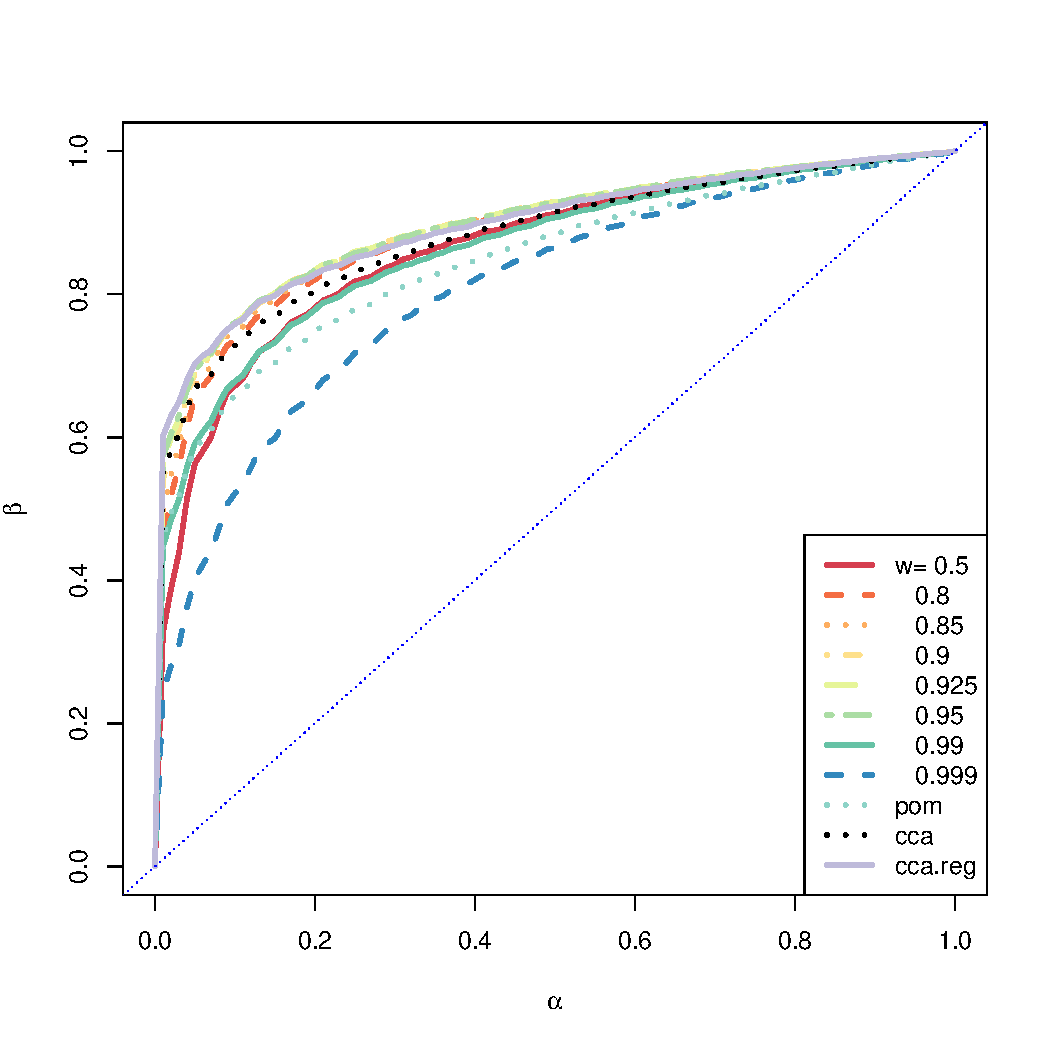
\includegraphics[scale=0.35]{MVN-FC-Tradeoff-OOS-c0_01.pdf}
\caption{Power ($\beta$) vs Type I error ($\alpha$) plot for different $w$ values for the Gaussian setting (noisy case)}
\label{fig:MVN-c001-power-alpha}
\end{figure}

\begin{figure}
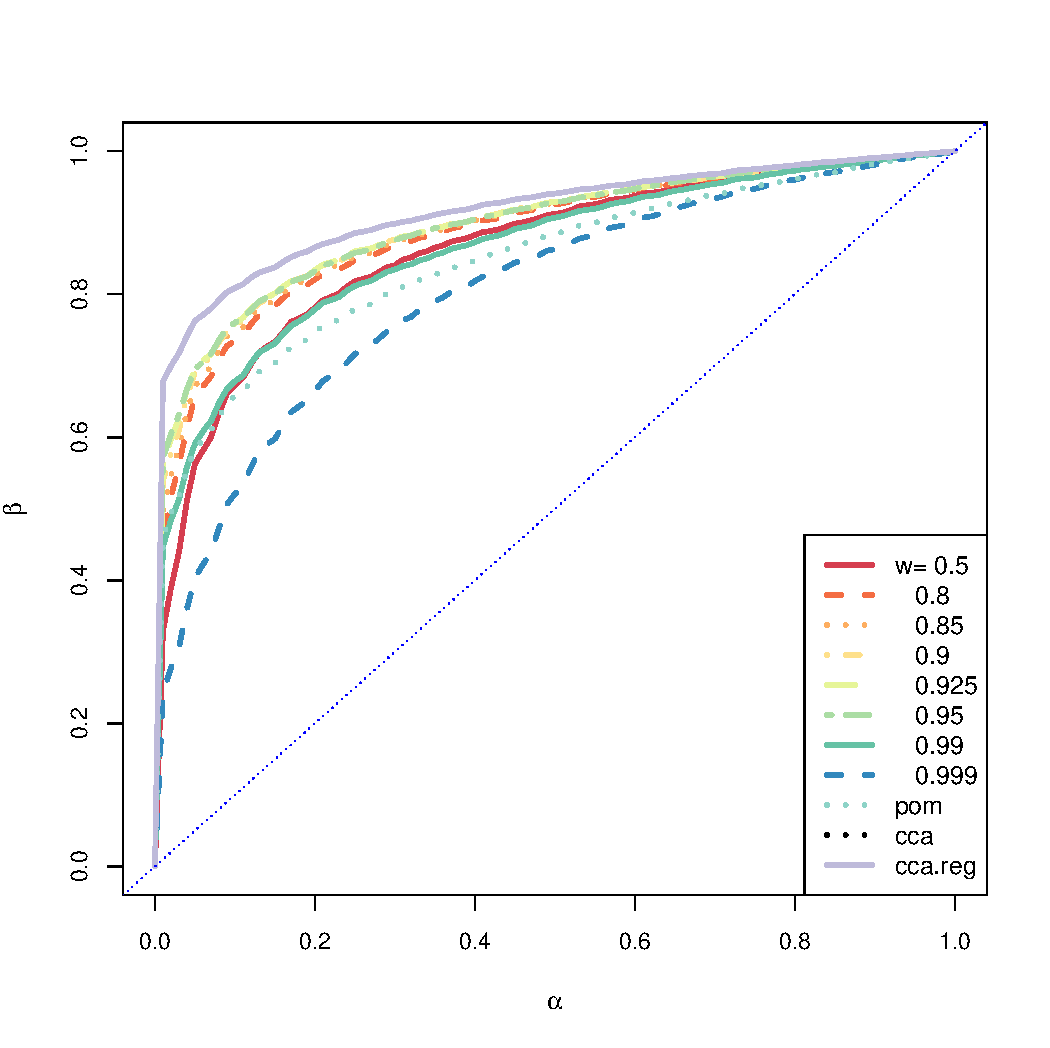
\includegraphics[scale=0.35]{MVN-FC-Tradeoff-OOS-c0.pdf}
\caption{Power ($\beta$) vs Type I error ($\alpha$) plot for different $w$ values for the Gaussian setting (noiseless case)}
\label{fig:MVN-c0-power-alpha}
\end{figure}

\begin{figure}
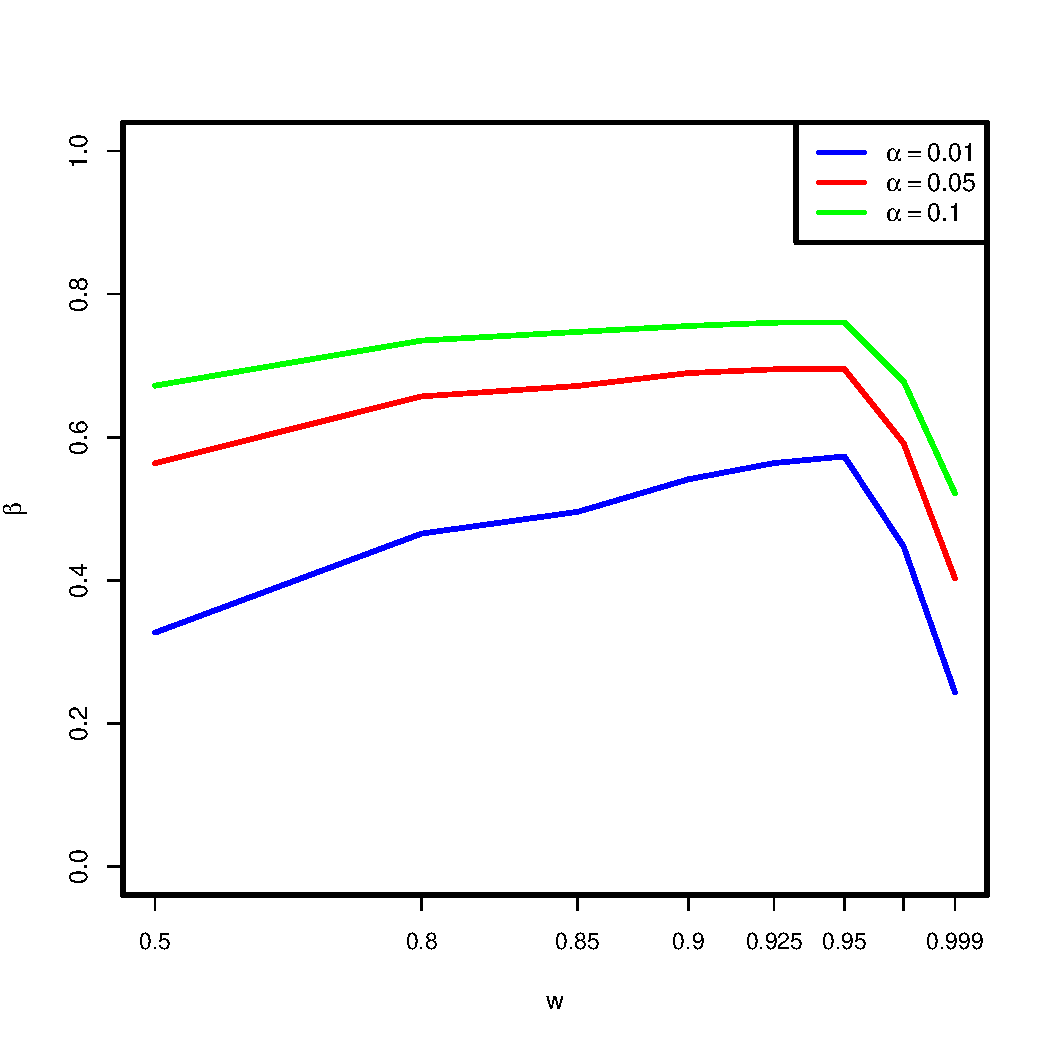
\includegraphics[scale=0.95]{OOSMVN-power-w-c0_01.pdf}
\caption{Power ($\beta$) vs $w$ plot for different Type I error ($\alpha$) values for the Gaussian setting (noisy case)}
\label{fig:MVN-c001-power-w}
\end{figure}


\begin{figure}
\includegraphics[scale=0.35]{Dirichlet-FC-Tradeoff-OOSc0-01-n150.pdf}
\caption{Power ($\beta$) vs Type I error ($\alpha$) plot for different $w$ values for the Dirichlet setting (noisy case)}
\label{fig:Dir-c001-power-alpha}
\end{figure}

\begin{figure}
\includegraphics[scale=0.35]{Dirichlet-FC-Tradeoff-OOSc0-n150.pdf}
\caption{Power ($\beta$) vs Type I error ($\alpha$) plot for different $w$ values for the Dirichlet setting (noiseless case)}
\label{fig:Dir-c0-power-alpha}
\end{figure}

\begin{figure}
\includegraphics[scale=0.95]{OOSDirichlet-power-w-c0-01.pdf}
\caption{Power ($\beta$) vs $w$ plot for different Type I error ($\alpha$) values for the Gaussian setting (noisy case)}
\label{fig:Dir-c001-power-w}
\end{figure}

Setting p and q to 5 and 10, respectively, for $n=150$ and $m=150$, the average of the power values for $nmc=150$ Monte Carlo replicates are computed at  different $\alpha$s and are plotted in Figure \ref{fig:MVN-c001-power-w} against $\alpha$ for the Gaussian setting.  Qualititatively similar plots for the Dirichlet setting  are not included for brevity.  The plot in Figure \ref{fig:MVN-c001-power-w} shows that for different values of  $w$, $\beta$-$\alpha$ curves vary significantly.  The conclusion is that the match detection tests with JOFC embedding using specific $w$ values have better performance than other $w$ values in terms of power.  In Figure
 \ref{fig:MVN-c001-power-w},  $\beta(w)$ is plotted against $w$ for fixed values of $\alpha$. It is  interesting that the optimal value of $w$ seems to be in the range of $(0.85,1)$ for all settings, which suggests a significant emphasis on commensurability might be  critical for the match detection  task. 




\begin{comment}
\begin{figure}
\includegraphics[scale=0.35]{OOS-MVN-power-w-c0.pdf}
\caption{$\beta$ vs $w$ plot for fixed $\alpha$ values for the Gaussian setting (noiseless case)}
\label{fig:MVN-c0-beta-w}
\end{figure}


\begin{figure}
\includegraphics[scale=0.65]{OOSMVN-power-w-c001.pdf}
\caption{Power ($\beta$) vs $w$ plot for fixed Type I error ($\alpha$) values for the Gaussian setting (noisy case)}
\label{fig:MVN-c001-beta-w}
\end{figure}

\end{comment}

Note that in Figure \ref{fig:MVN-c001-power-w} for $\alpha=0.05$, $\beta_{\alpha=0.05}(w=0.99)\geq\beta_{\alpha=0.05}(w=0.5)$. However, for $\alpha=0.3$, $\beta_{\alpha=0.3}(w=0.99)\leq\beta_{\alpha=0.3}(w=0.5)$. This justifies our comment that  $w^{*}$  must be defined with respect to $\alpha$.


\begin{comment}
\begin{figure}
\includegraphics[scale=0.35]{OOS-Dirichlet-power-w-c0.pdf}
\caption{$\beta$ vs $w$ plot for fixed $\alpha$ values for the Dirichlet setting(noiseless case)}
\label{fig:fig7}
\end{figure}

\begin{figure}
\includegraphics[scale=0.35]{OOS-Dirichlet-power-w-c0-01.pdf}
\caption{$\beta$ vs $w$ plot for fixed $\alpha$ values for the Dirichlet setting(noisy case)}
\label{fig:fig8}
\end{figure}
\end{comment}



Note that  for all of the settings, the estimate of the optimal $w^{*}$ has  higher power than $w$=0.5 (the unweighted case).
To test the statistical significance of this observation,   the null hypothesis that  $H_{0}: \beta_{\alpha}({\hat{w}^*})\leq\beta_{\alpha}({w=0.5})$  is tested against the alternative $H_{A}=\beta_{\alpha}({\hat{w}^*})>\beta_{\alpha}({w=0.5})$.  The least favorable null hypothesis is that  $H_{0}: \beta_{\alpha}({\hat{w}^*})=\beta_{\alpha}({w=0.5})$.
Using previous notation,  the test statistic will be denoted by $T_a(w)$ under the alternative hypothesis and $T_0(w)$ under the null hypothesis.

McNemar's test will be used to compare the two predictors (referred to as $C_1$ and $C_2$ with $w$=0.5 and $w$=$w^*$ at a fixed $\alpha$ value.

For a fixed $\alpha$ value, one can compute two critical values $c(0.5)=max_l \{  P(T_0(0.5)>c)<\alpha\}$,  $c(w^*)=max_l \{  P(T_0(w_2)>c)<\alpha\}$. The values of the decision function that uses these critical  values, for each pair of embedded points (indexed by $i$, are  $(\tilde{y}_i^{(1)},\tilde{y}_i^{(2)}),\hspace{7pt}i=1,\ldots,m$. To compare the  two statistical tests with  $w=0.5$ and $w$=$w^*$  , one can prepare a $2\times 2$ contingency-table of correct decisions and incorrect decisions made by each statistical test (or equivalently true and false classifications made by two classifiers). Denote decision outcome as $g_1$ for the first statistical test and $g_2$ for the second statistical test. If $g_1=True$ and $g_2=False$ for an instance,  the first test made the correct decision and the second test made the incorrect decision with regard to the null and alternative hypotheses.
% McNemar's test was used to compare the two contingency tables for fixed $\alpha$. McNemar's test is a statistical test for %comparing two binary classifiers based on a 2-by-2 table of the counts of misclassifications of each. That is,
Consider the contingency table for a Monte Carlo replicate given by $$G^{(l)}= \begin{array}{|c|c|}
      \hline
       e_{FF}^{(l)} & e_{TF}^{(l)}\\
      \hline
       e_{FT}^{(l)} & e_{TT}^{(l)}\\
      \hline
      \end{array}      $$  where $l$ is the index of the MC replicate, $e_{g_1g_2}^{(l)}$ is equal to the number of instances at which the true hypothesis were identified  correctly ($g_1=True$) or incorrectly ($g_1=False$) by the first test, and correctly ($g_2=True$) or incorrectly ($g_2=False$) by the second test in that MC replicate.

Under the null  hypothesis that the two predictors have the same power at $\alpha$ ,
 $Pr[\left(g_1g_2\right)=(TF)]=Pr[\left(g_1g_2\right)=(FT)]$, so $\sum_l{I \{e_{TF}^{(l)}>e_{FT}^{(l)}\}}$ will be distributed according to  the binomial distribution, $\mathcal{B}(nmc,0.5)$. ($I\{\cdot\}$ is the indicator function.) 

% For each Monte Carlo replicate, the p-value of McNemar's test was computed separately.

\begin{comment}
\begin{figure}
\begin{tabular}{p{4.7cm}p{4.7cm}}
$e_{00}$:Misclassified by \newline Both $C_1$ and $C_2$ & $e_{10}$:Correctly Classified by $C_1$,\newline Misclassified by $C_2$\\
& \\
$e_{01}$:Correctly Classified by $C_1$, \newline Misclassified by $C_2$ & $e_{11}$:Correctly Classified by \newline Both $C_1$ and $C_2$
\end{tabular}. 

\caption{Contingency Table for McNemar's test for comparing two classifiers, $C_1$ and $C_2$}
\label{fig:cont-table}
\end{figure}
\end{comment}

For the noisy version of the Gaussian setting at allowable type I error 0.05 for the two tests, when comparing  the null hypothesis that  $H_{0}: \beta_{\alpha}({\hat{w}^*})=\beta_{\alpha}({w=0.5})$ against the alternative $H_{A}=\beta_{\alpha}({\hat{w}^*})>\beta_{\alpha}({w=0.5})$, the p-value is $p<1.09E-24$ which indicates the power using estimate of optimal $w^*$ is significantly greater than the power when using $w=0.5$. 
%In fact
% the distribution of p-values from McNemar's tests is skewed and  we reject $\beta_{0.5}>=\beta_{w^*} $ for  55\%  of the %Monte Carlo replicates.


 Another avenue for investigation is  how the parameters of the distribution of  data such as $p$ ,$q$, $r$, $c$ and $d$ affect the results. For example, it was  speculated that as $q$, the number of   ``noise" dimensions increases, the performance of  CCA approach would suffer, due to spurious correlations. This hypothesis was tested using simulated data with q=90. The  bundle of ROC curves in the Figure \ref{fig:largeq}.  Both CCA and  regularized CCA is not competitive with JOFC approach with the appropriate $w$ values. In fact, the ROC curve for CCA is not very distinct from  random guess line.

\begin{figure}
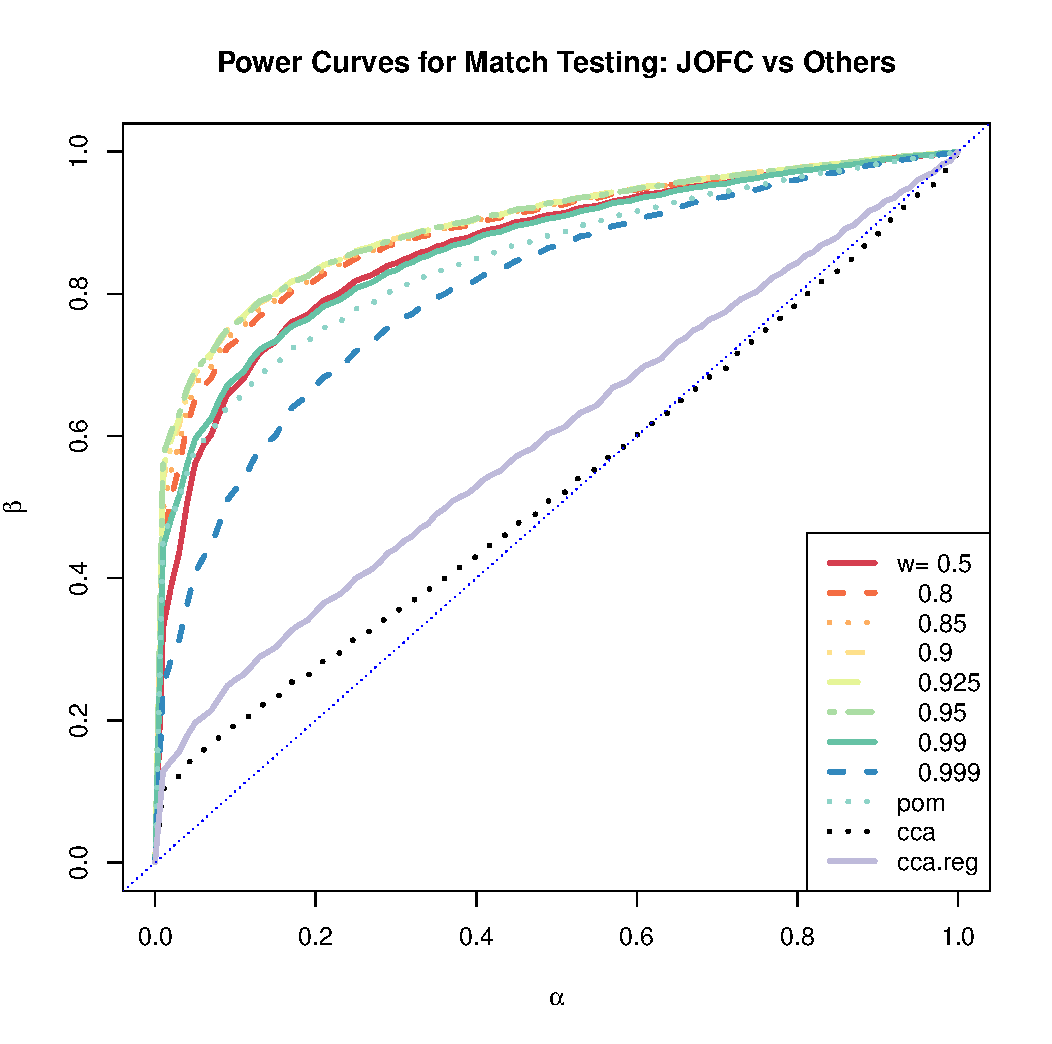
\includegraphics{MVN_JOFC_q_90_c_0_001}
\caption{}
\label{fig:largeq}
\end{figure}


\begin{comment}



The same pair of plots are included for various values of parameters $p$,$q$ ,$r$ and $c$.

Speculation on the effects of parameters in Gaussian/ Dirichlet settings

 Another avenue for investigation is  how $w^{*}$ depends on the parameters of the distributions of $\mathbf{F}_m$ and  $\mathbf{F}_u$ . 
 Let us first investigate the effect of parameters on the empirical distribution of the test statistic, under null and alternative.
 For our Multivariate Normal and Dirichlet models, consider the signal and noise dimensions $p$ and $q$ respectively.
  An increase in $p$ leads to the inflation of the test statistic under alternative  \ref{fig-stats-p},
it also effects the distribution of the test statistic under null. As $p$ increases, the probability of getting a new dimension in the matched vectors
 in which the matched pairs are highly correlated increases.  


 So any $w$ value that takes advantage of this situation and  are small enough to preserve fidelity, yet large enough to not lose significantly from commensurability will have increases in power to become $w^*$. 




Consider  an increase in $r$, this will cause the test statistic under null to be stochastically smaller,
 leading to a smaller critical value. So , a increase in priority of fidelity,
  which corresponds to smaller $w$ might lead to the inflation of the test statistic under alternative, and therefore an increase in power.\ref{fig-stats-r}  




Consider increases in $c$, which will increase the dissimilarity  both between matched and between unmatched vectors. 







Consider increases in $q$,  the test statistic under both null and alternative is inflated\ref{fig-stats-q}. 


 If commensurability can be preserved in the face of the increase in $q$, the power of the test may be preserved. However a very large increase in $w$ is not guarenteed to increase the preservation of commensurability, since the extra dimensions are noise, trying to   make the differences between coordinates  small in those dimensions will not  help in power, in fact may be disruptive since,
  more fidelity may be lost in the effort to bring the pair of points together.





\end{comment}



\section{Experiments on Wiki Data}
To test the JOFC approach with real data, a collection of articles are collected from the English Wikipedia, consisting of the
 directed 2-neighborhood of the document "Algebraic Geometry". 
   This  collection of 1382 articles and the correspondence of each article in French 
Wikipedia is our real-life dataset. It is possible to utilize both textual content of the documents and the hyperlink graph structure. The textual content of the documents is summarized by the bag-of-words model. Dissimilarities between documents  in the same language are computed by the Lin-Pantel discounted mutual information \cite{LinPantel,PantelLin}
 and cosine dissimilarity $k(x_{ik}; x_{jk}) = 1 - (x_{ik} x_{jk})/(\|x_{ik}\|_2\|x_{ik}\|_2)$. 
 The dissimilarities based on the hyperlink graph of the collection of the articles are 
 for each pair of vertices $i$ and $j$, the number of vertices one must travel to go from $i$ to $j$.  Further details about this dataset is available in \cite{Zhiliang_disparate}     
Only  dissimilarities based on the textual content will be considered in this example.
   
The exploitation task is still testing for matchedness of vertices between different conditions, in this case wiki articles that are on the same topic  in  different languages.
For hypothesis testing,   randomly held out four documents - one matched pair and one unmatched pair
 -  are used to compute empirical type I error $\alpha$ and estimate of power based on the critical value computed
  from the distribution of the test statistic for the remaining 1380 matched pairs. 
The test statistic is computed using one of the three approached mentioned  $cca$, $p\circ m$, and $jofc$ . 
The two sets of held-out matched pairs are embedded as $\tilde{y}_1$ and $\tilde{y}_2$, via out-of-sample
embedding, to estimate the null distribution of the test statistic $T = d(\tilde{y}_1; \tilde{y}_2)$. This allows
us to estimate critical values for any specified Type I error level. 
Then the two sets of heldout unmatched pairs are embedded as $\tilde{y'}_1$ and $\tilde{y'}_2$, via out-of-sample embedding. 
$T' = d(\tilde{y'}_1; \tilde{y'}_2)$ will give us an empirical distribution of the test statistic  under the alternative hypothesis. 
And the distribution under null hypothesis and under alternative hypothesis can be used to estimate power.
Target dimensionality d is determined by the Zhu and Ghodsi  automatic dimensionality selection
method \cite{ZhuGhodsi}, resulting in d = 6 for this data set.


\includegraphics{graphs/FidCommPaperwiki-two-cond-plot} 



\section{Model Selection}
For the simulations presented up to now, the embedding dimension $d$ was set to 2. This was a convenient choice which allowed us to investigate various aspects of JOFC and competing approaches.
However,  more care is required in selection of this parameter, since it plays such a big role in performance in general learning settings. The signal dimension was set to $p=10$ and different $d=2,5,7,10,15$ values were used to test the JOFC approach.
The following plots of ROC curves in    \ref{fig:ROC-d} and  \ref{fig:ROC-d-15} shows the effect of $d$ parameter on the performance of different methods for the Gaussian setting for the noisy case. 
\begin{figure}
 \centering
  \captionsetup[subfigure]{labelformat=empty}
        \begin{subfigure}[b]{0.5\textwidth}        
               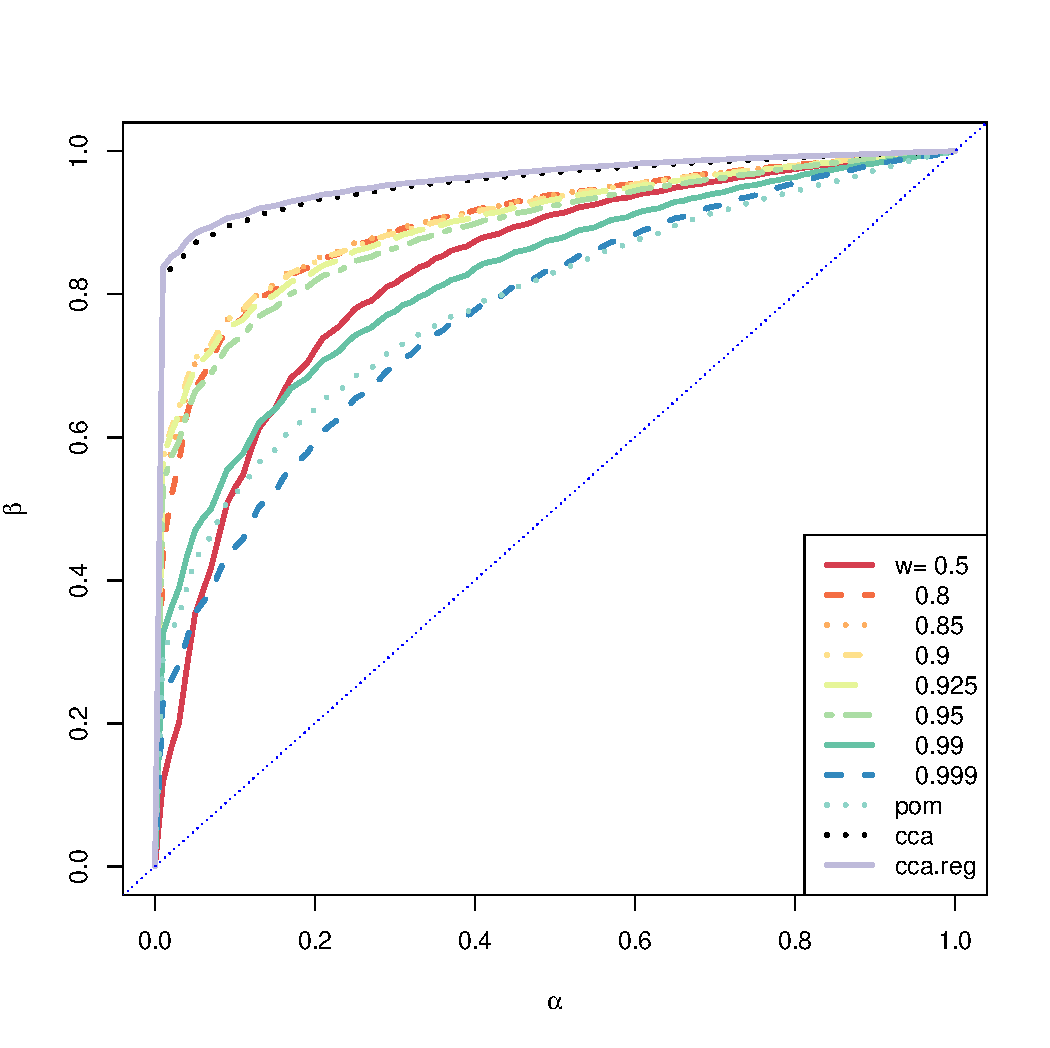
\includegraphics[width=\textwidth]{ROC-d-2.pdf}
                \caption{d=2}
                \label{fig:ROC-d-2}
        \end{subfigure}%
         %add desired spacing between images, e. g. ~, \quad, \qquad etc. 
          %(or a blank line to force the subfigure onto a new line)
        \begin{subfigure}[b]{0.5\textwidth}           
                  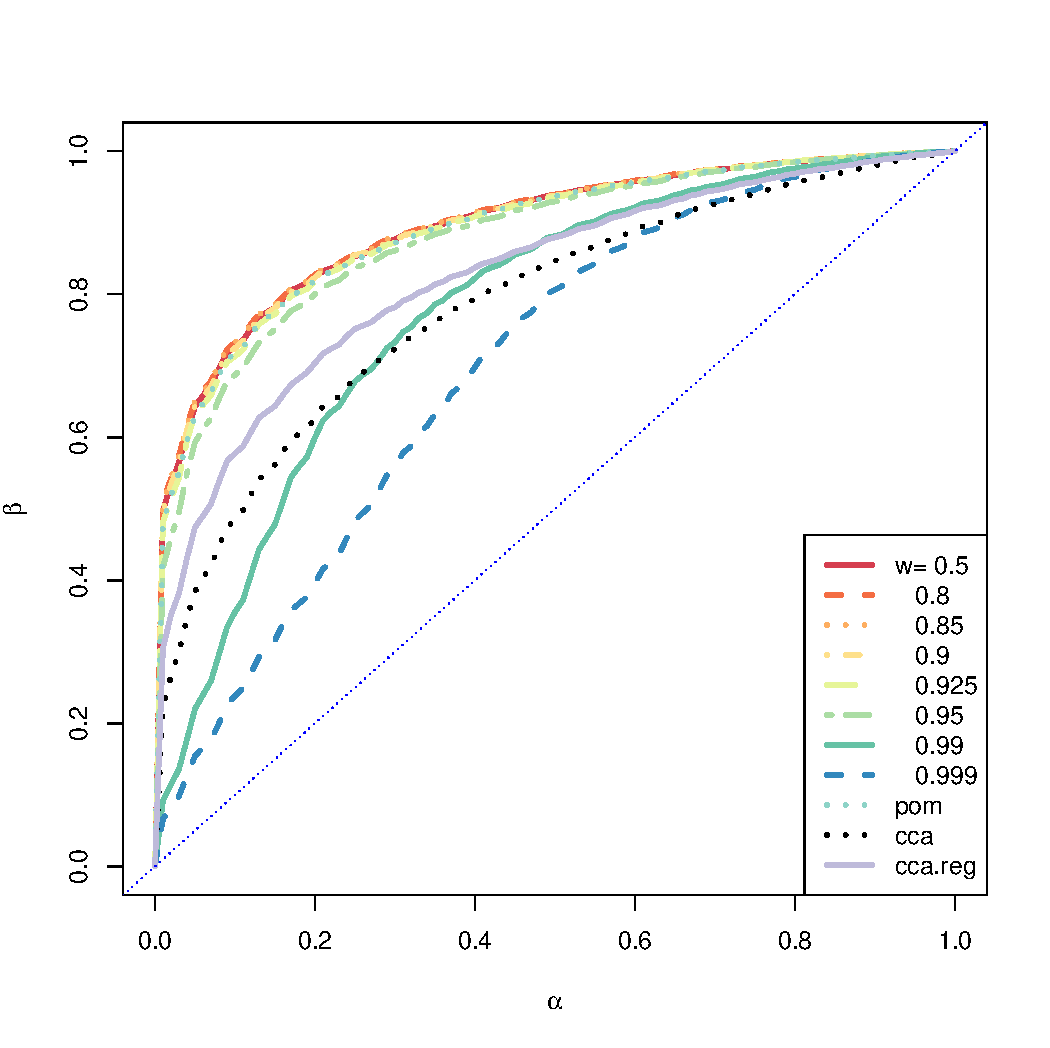
\includegraphics[width=\textwidth]{ROC-d-5.pdf}
                \caption{d=5}
                \label{fig:ROC-d-5}
        \end{subfigure}      
        %add desired spacing between images, e. g. ~, \quad, \qquad etc.    %(or a blank line to force the subfigure onto a new line)
        \begin{subfigure}[b]{0.47\textwidth}             
               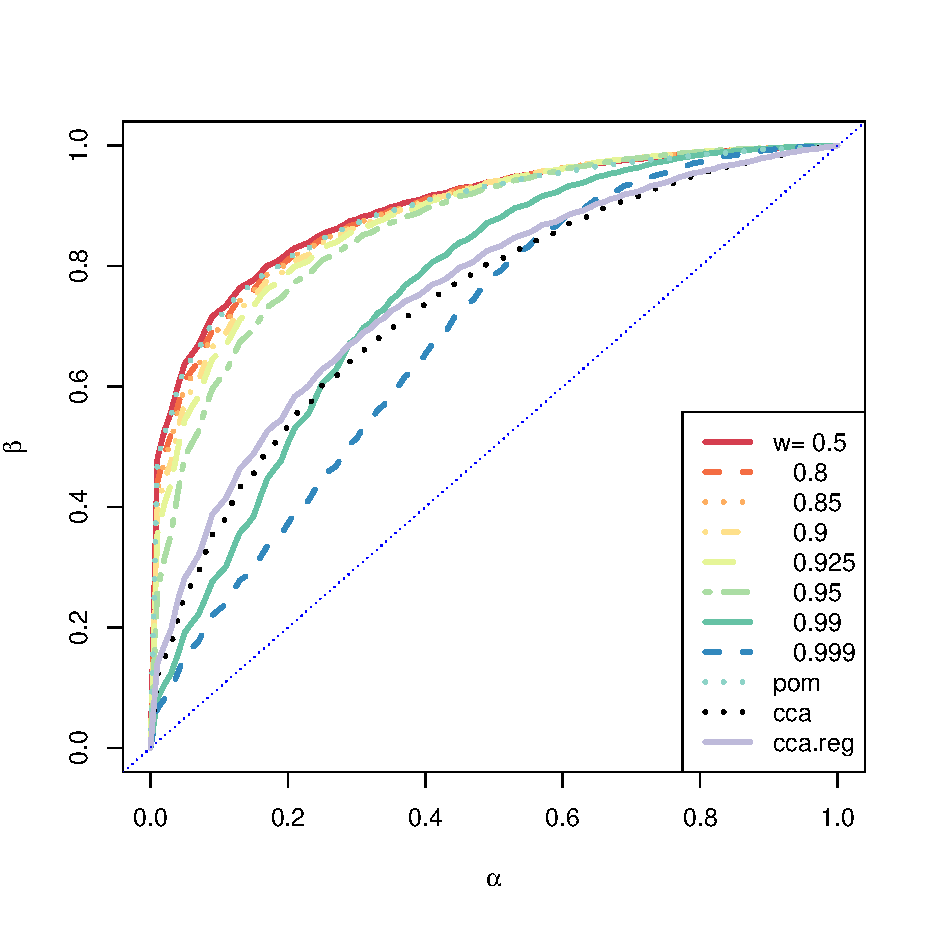
\includegraphics[width=\textwidth]{ROC-d-7.pdf}
                \caption{d=7}
                \label{fig:ROC-d-7}
        \end{subfigure}          
               \begin{subfigure}[b]{0.47\textwidth}
                \centering
               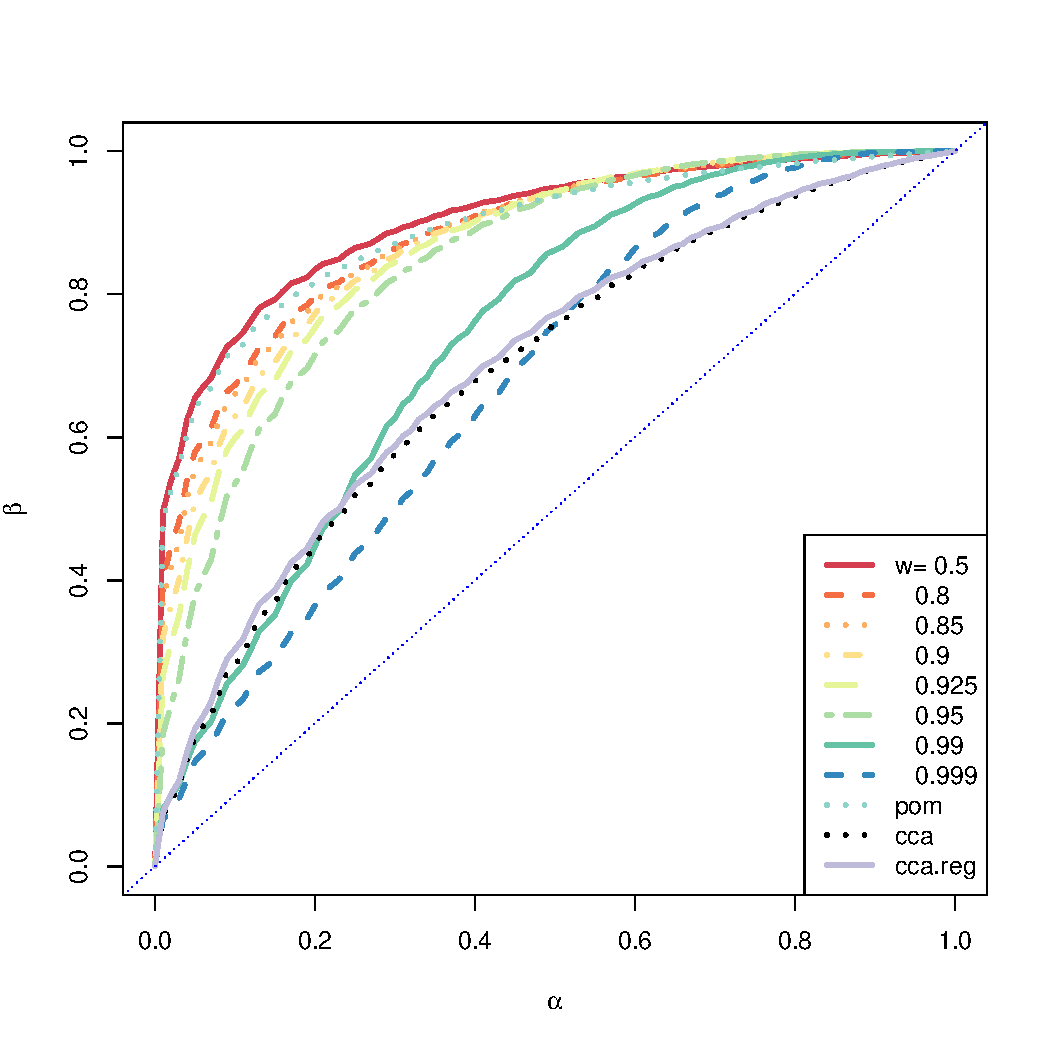
\includegraphics[width=\textwidth]{ROC-d-10.pdf}
                \caption{d=10}
                \label{fig:ROC-d-10}
        \end{subfigure}
         
        \caption{Effect of $d$ parameter on ROC plots}\label{fig:ROC-d}
        \label{fig:ROC-d}

\end{figure}
\begin{center}
\begin{figure}

                \centering
               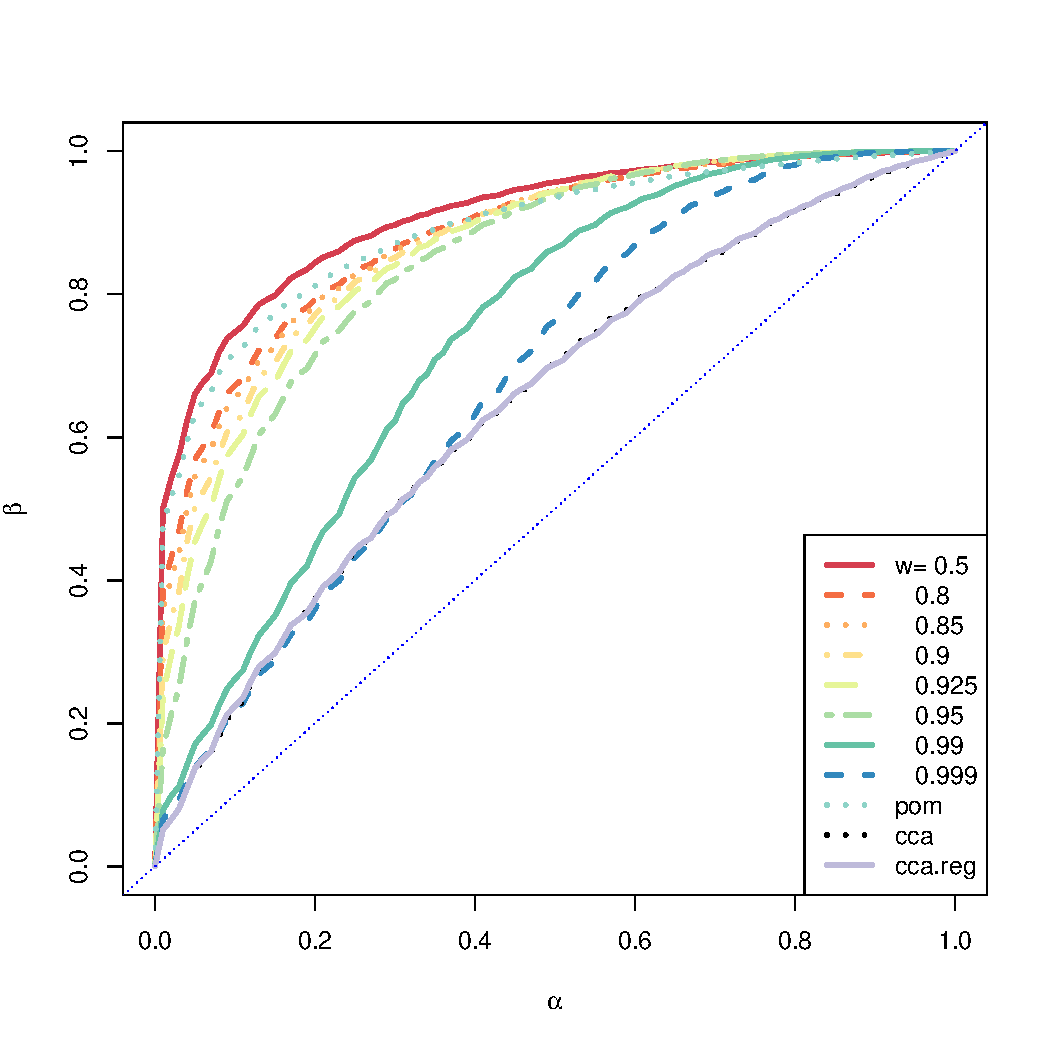
\includegraphics[scale=0.3]{ROC-d-15.pdf}
                \caption{d=15}
                \label{fig:ROC-d-15}
       
\end{figure}
\end{center}








\section{Experiments on Graph Data}

Another application of  the JOFC approach to  the vertex matching problem in multiple graphs. These simulations will be for the same semi-supervised setting as mentioned in \ref{sec:RelatedWork}, where matchings between some vertices in different graphs are known 
  and the task is to infer the correspondences between the remaining collection of vertices in the graphs. The pairs of vertices whose correspondences are known will be referred to as ``seeds''.

Suppose $A,B \in \mathcal{R}^{(r+s)\times (r+s)}$ are adjacency matrices for graphs 
 partitioned as ($r$ rows then $s$ rows, $r$ columns then $s$ columns)
\[  A =\left [
\begin{array}{cc} A_{11} & A_{12} \\ A_{21} & A_{22} \end{array} \right ]
\ \ \ \ \ \ \ \ \ B =\left [
\begin{array}{cc} B_{11} & B_{12} \\ B_{21} & B_{22} \end{array} \right ]
\]
To simplify  suppose that $A_{11}=B_{11}$ , ie the first $r$ vertices
of $A$'s graph correspond respectively to the first $r$ vertices of $B$'s graph,
and we wish to complete the isomorphism by determining the correspondences between the pairs of $s$ vertices. 
That is, we seek a permutation matrix $P \in \{0,1\}^{s \times s}$ such that $A=(I_{r \times r}
\oplus P)B(I_{r \times r} \oplus P)^T$, ie
 \[
 \left [
\begin{array}{cc} A_{11} & A_{12} \\ A_{21} & A_{22} \end{array}
\right ]
\left [
\begin{array}{cc} I_{r \times r} & 0_{r \times s} \\ 0_{s \times r} & P \end{array}
\right ]
=
\left [
\begin{array}{cc} I_{r \times r} & 0_{r \times s} \\ 0_{s \times r} & P \end{array}
\right ]
\left [
\begin{array}{cc} B_{11} & B_{12} \\ B_{21} & B_{22} \end{array}
\right ] .
\]

Using omnibus  embedding, it is possible to embed the vertices of two graphs in a commensurate space.
Therefore, the JOFC approach can be used here for determining the pairwise distances between  the vertices of $A$ and $B$.
The next step is to use the pairwise distances to find the optimal 1-1 matchings by the Hungarian algorithm \cite{Hung-algo}. The Hungarian algorithm finds an optimal matching between two sets of vertices such that the total  cost which is the sum of the pairwise distances of matched nodes is minimized.
 
One useful property of dissimilarity representation is that the structure of data is irrelevant once an appropriate dissimilarity function  for the data is available. 
There are many distances that can be defined between vertices in graphs. We assume that an appropriate distance measure is available to us.
In our experiments we will use three different dissimilarities between vertices in a graph:
\begin{itemize}
 \item the shortest path on the  unweighted graph whose adjacency matrix is available
 \item the shortest path on a weighted version of the graph whose adjacency matrix is available
 \item diffusion distance between vertices on the (unweighted) graph.
 \item weighted extension of Czekanowski-Dice dissimilarity\cite{DICE,weightedDICE} which simplifies to the original Czekanowski-Dice dissimilarity (C-D dissimilarity  quantifies local similarity of two vertices in a graph).
 \end{itemize}
 We will omit the results for weighted graph dissimilarities, since they seem to have the same performance as the weighted dissimilarities.
 
 Note that these dissimilarities can only be defined between vertices of the same graph. We impute the inter-condition dissimilarities   as described before in section \ref{omnibus}.
 
  To test JOFC approach, consider the following simulation: $A$ is the adjacency matrix of an Erdos-Renyi graph, that is
  $\left[A\right]_{ij} \sim Binomial(p)$ where $\left[A\right]_{ij}$ is $ij$-th entry of the adjacency matrix  $A$.
   and the adjacency matrix  $B$ is a entry-wise bit-flipped version of the adjacency matrix of $A$, that is
   In the following simulation, $A$ is the adjacency matrix of an Erdos-Renyi graph, that is
  $\left[A\right]_{ij} \sim Binomial(p)$ where $\left[A\right]_{ij}$ is $ij$-th entry of the adjacency matrix  $A$.
   and the adjacency matrix  $B$ is a entry-wise bit-flipped version of the adjacency matrix of $A$, that is
   $\left[B\right]_{ij}|\left[A\right]_{ij}=0 \sim Binomial(p_{10})$ $\left[B\right]_{ij}|\left[A\right]_{ij}=1 \sim Binomial(p_{11})$. Suppose $p_{10}=p_{11}=p$.
  
  The probability of flipping an entry of the adjacency matrix is the perturbation parameter $p_{pert}$ which is the variable on the x-axis. 
  The performance measure is the proportion of true matches to the number of matches. Note that 
  under chance, the expected number of true matches is 1, as shown with the dashed line. In the simulation, $r=20$ and $s=5$. $p_{pert}$ varies from $0$ to $1$ in increments of $0.1$. 
	
\begin{figure}
  \includegraphics[scale=0.65]{FidCommPapergraph-plot-1.pdf}
\end{figure}


In the plot above, JOFC approach is used to find  matched pairs of vertices using  dissimilarities based on weighted and unweighted graphs and  compared with classical MDS embedding of dissimilarities of weighted graphs.

Note that JOFC for unweighted and weighted graphs  have better performance compared to CMDS. As the perturbation parameter gets larger, the performance degrades until it is indistinguishable from random chance at $pert=0.5$.

\begin{comment}
Another feature of the plot is the U-shape of the curve for diffusion-distance based dissimilarities. This invariancy with respect to complement of the graph should be investigated further.

\includegraphics{graphs/FidCommPapergraph-plot-3}An interesting trend in the graph is that shortest-path based dissimilarities are an improvement over diffusion-path dissimilarities for perturbation parameter less than 0.5 , but as perturbation parameter increases past 0.5, fraction of correct matches for diffusion distance based dissimilarity recovers, while for other dissimilarities the fraction continues to fall. 
\end{comment}




This graph shows the effect of the weight parameter of stress $w$ on the probability of true matches.

\includegraphics{FidCommPaper-graph-plot-4}

There are a lot  of interesting questions to ponder about the number of known correspondences, such as , how many known correspondences are necessary for satisfactory performance for graphs of some fixed size and whether , in the ``match ratio'' vs number of known correspondences curve,  there are any ``elbows'' , after which the cost of more correspondences are not justified by the accompanying increase in ``match ratio''. Figure \ref{bitflipJOFC} shows ``match ratio'' plotted against number of ``seeds'' for the same bitflip experiments using  Czekanowski-Dice dissimilarities . These results suggest that even with the perturbation, when a portion of the correspondences are known, it is possible to recover most of the remaining correspondences. This application of JOFC is  investigated further in \cite{SGMviaJOFC} with real datasets.
\begin{figure}
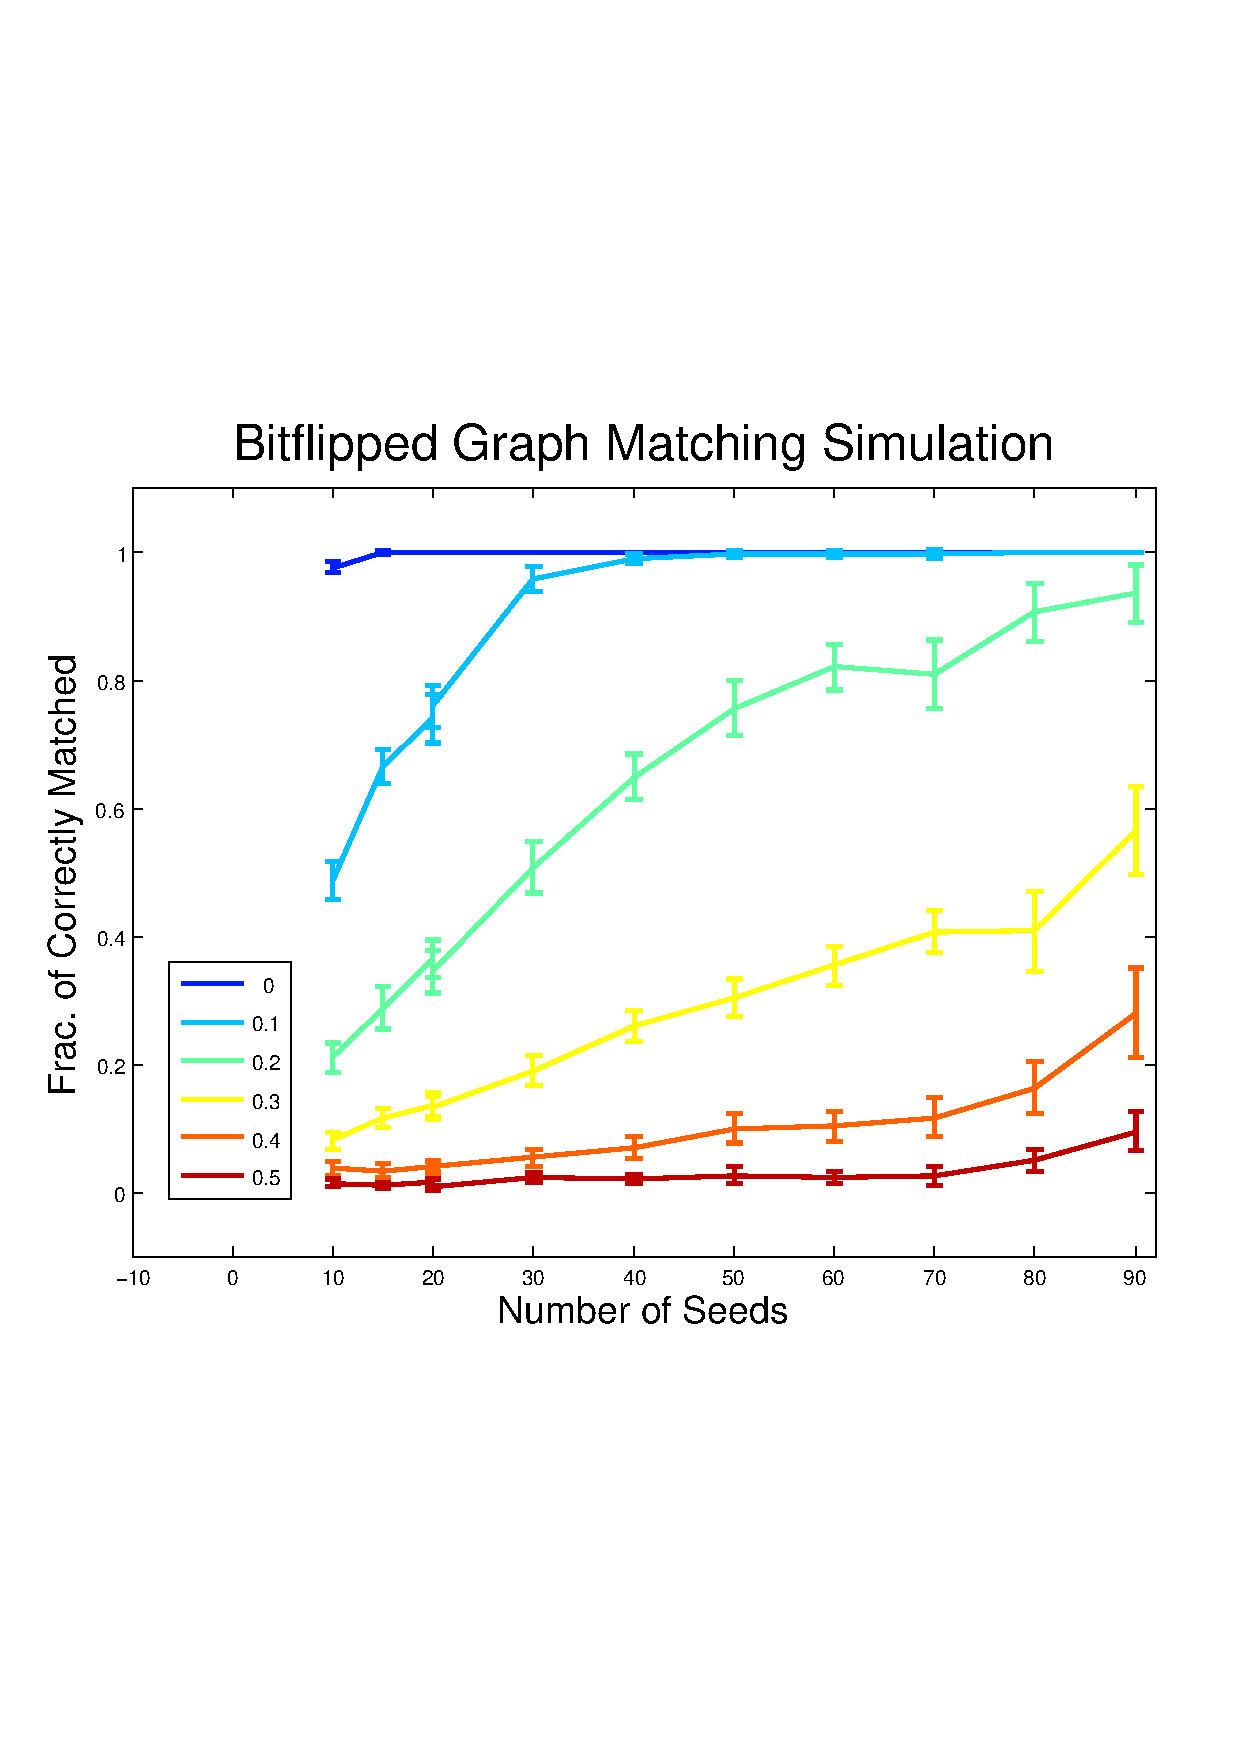
\includegraphics{bitflip_JOFC}
\caption{Bitflip Simulations for JOFC \label{bitflipJOFC}}
\end{figure}




\chapter{Multiple Minima in  Multidimensional Scaling }
\label{sec:MultMinima}
\chaptermark{Optional running chapter heading}


\subsubsection{ A short detour : Discontinuity in weighted raw stress OOS configurations\label{subsubsec:Discontinuity}}

Note that it is possible to have multiple local minima in the embedding step(see example in \cite{TrossetLocalMin}). It is also possible to construct an example  where the weight parameter $w$ controls which of the local minima is the global minimum among the configurations of $\hat{X}_{.}$.

%Global Minimum Configuration determined by $w$ .

Consider five in-sample points in $\mathbb{R}^2$ with locations $X_1=(0,0)$, $X_2=(1,0)$, $X_3=(1,1)$
 and $X_4=(1,0)$, $X_5=(.5,.5)$ and two out-of-sample  points with coordinates $X_6=(1,0)$ and $X_7=(0,1)$.
 \begin{figure}
 \centering
 \includegraphics[scale=0.35]{multmin-diag}
 \caption{True configuration of $X_{i}$, $i \in {1,\ldots,7}$}
\label{original-config}
 \end{figure} 
  Suppose $X_6$ is matched with $X_2$ and $X_7$ is matched with $X_4$. 
  Denote the Euclidean distance matrix by $D$. 
  Suppose, due to noise, or due to dissimilarities not being Euclidean distances, 
  the dissimilarity matrix is $$D'_{ij}=\begin{cases}
  D_{ij}-1.4 & \textrm{if  $(i,j) \in \{(4,6),(6,4),(2,7),(7,2)   \}$ }\\
  D_{ij}  & \textrm{ otherwise}\\
  \end{cases}.$$ 
Qualitatively, the three points $X_1$, $X_5$ and $X_3$ form a barrier which the OOS points need to cross  to reach their matched counterparts. 

The MDS criterion function is optimized starting with different initial configurations.   Depending on the initial configuration, the final embedding coordinates of $\hat{X}_6$ might be closer
    to $X_4$ compared to $X_2$. This is due to a local minimum in the configuration space. Consider the fact that, at the start of optimization, if  the initial coordinates of $\hat{X}_6$ is on the $X_4$ side of the $y=x$ line  in  $\mathbb{R}^2$ , 
    it has to cross paths with the embeddings of  ${X}_1,{X}_3,{X}_5$ and it has   nonzero dissimilarities with those points. The same argument can be made for $X_7$. This is  the ``barrier" mentioned that is encountered in the optimization. It is possible to distinguish two kinds of local minima, one where the embedded OOS points $X_6$ and $X_7$ end up in the same side as their respective matched points $X_2$ and $X_4$ (named ``true'' or real config.) and the other where they end up in sides  opposite their matched points (named ``alternative" local min.). The latter corresponds to the case where the OOS points are unable to cross the ``barrier"'. Other configurations such as the ones where $X_6$ and $X_7$  end up in the same side are not local minima, since the original dissimilarity between them is large ($\sqrt{2}$) compared to dissimilarities between other pairs of points and embedding them close would increase raw stress significantly.
    Based on value of $w$, it might be easier to get out of the  ``alternative" local minimum. 
    In addition, depending on $w$ , this  local minimum can be a global minimum. 
    That is, if $w$ is small enough, the configuration where $X_6$ stays on the side of $X_4$ instead of $X_2$ might have a lower stress than the configuration where $X_6$ is near its matched point $X_2$, due to the fact that  contribution of $ D_{ij}-d(X_i,X_j)$ to the raw stress where $(i,j)=(4,6)$  is  multiplied by $1-w$ while every other dissimilarity is multiplied by $w$. 
		
		Starting from a small enough $w$ and increasing it until $w$ is arbitrarily close to $1$, there are two $w$ values where important changes in embedding configurations and final stress values occur.
    The plots in Figures \ref{fig:Finalconfig-MultMin-w-0_1}, \ref{fig:Finalconfig-MultMin-w-0_5}, \ref{fig:Finalconfig-MultMin-w-0_8}, \ref{fig:Finalconfig-MultMin-w-0_81} , \ref{fig:Finalconfig-MultMin-w-0_84} show the local minimum configurations ${X}_6$(in red circles) and ${X}_7$(in blue plusses) end up in starting from different initial configuration(One red and one blue point for each  initial configuration) The point pairs plotted in the left box are those configurations  where the  ${X}_6$ and ${X}_7$ end up in the side of their matched points (``true'' final configuration). The configurations in the right are those where the points end up in the opposite side of their matched points. The final stress values of the final configurations listed in  \ref{stress-val-table} (the minimum stress value among each kind of local minima) show that around $w=0.5$ the  ``true''-kind local minima   starts having a lower stress value compared to ``alternative''-kind. This is the first $w$ value that corresponds to an important change. Also note that starting around $w=0.8$ in Figure \ref{fig:Finalconfig-MultMin-w-0_8}, all of the $X_5$ and $X_6$  pairs are on the verge of passing throught the barrier and start ending up in the side of their matched points, due to the fact that the barrier starts to become negligible and there are no separate local minima. When $w>0.8$ all of the point pairs end up in  the``real'' configuration \ref{fig:Finalconfig-MultMin-w-0_81}. This is the $w$ value where the other important changes in configurations and stress values occur. Further increasing $w$ changes the final stress value, and  the final embedding configuration moves closer to the original locations of $X_{i}$ in \ref{original-config} \ref{fig:Finalconfig-MultMin-w-0_84}.
    


\begin{figure}
\begin{minipage}[b]{0.5\linewidth}
\centering
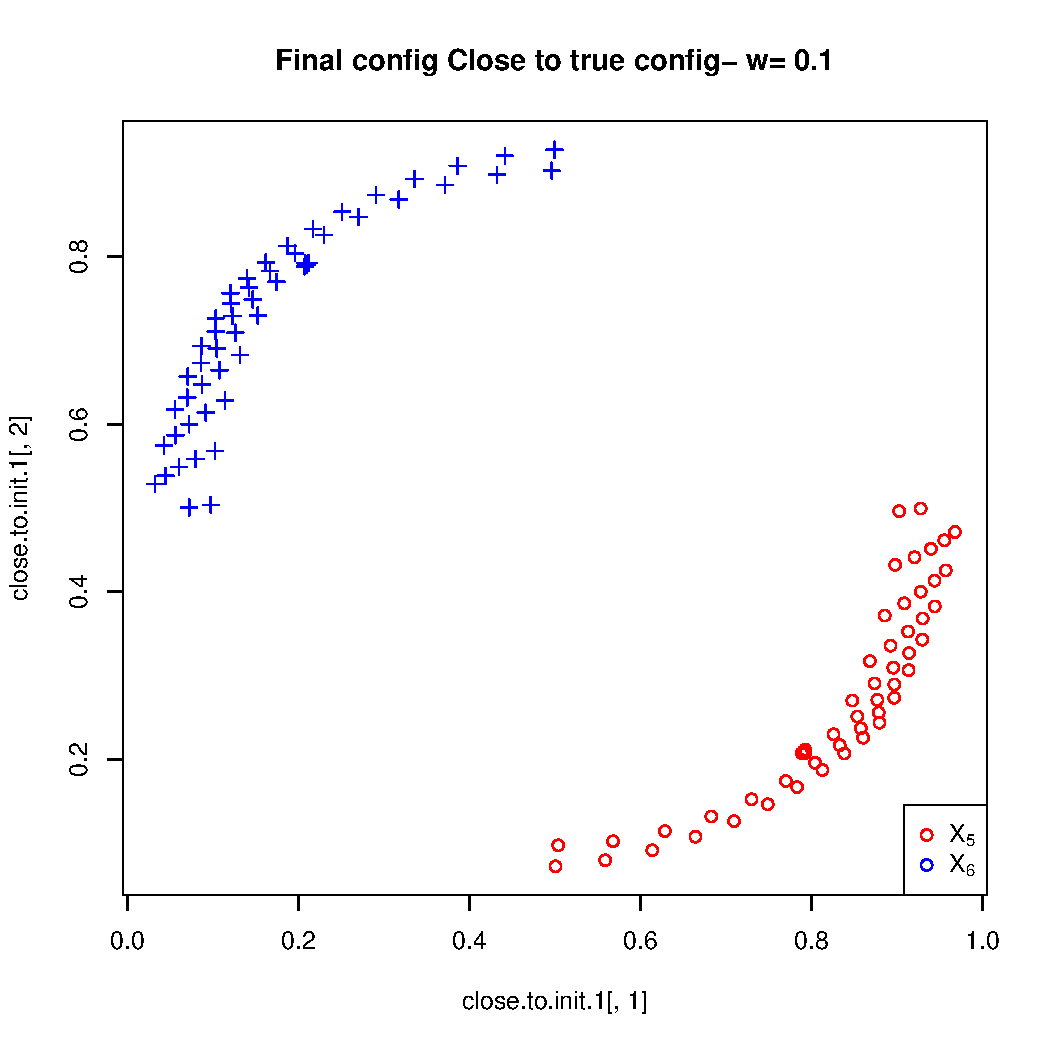
\includegraphics[scale=0.35]{true-min-w-0_1.pdf}

\label{fig:Finalconfig-MultMin-w-0_1_a}
\end{minipage}
\hspace{0.5cm}
\begin{minipage}[b]{0.5\linewidth}
\centering
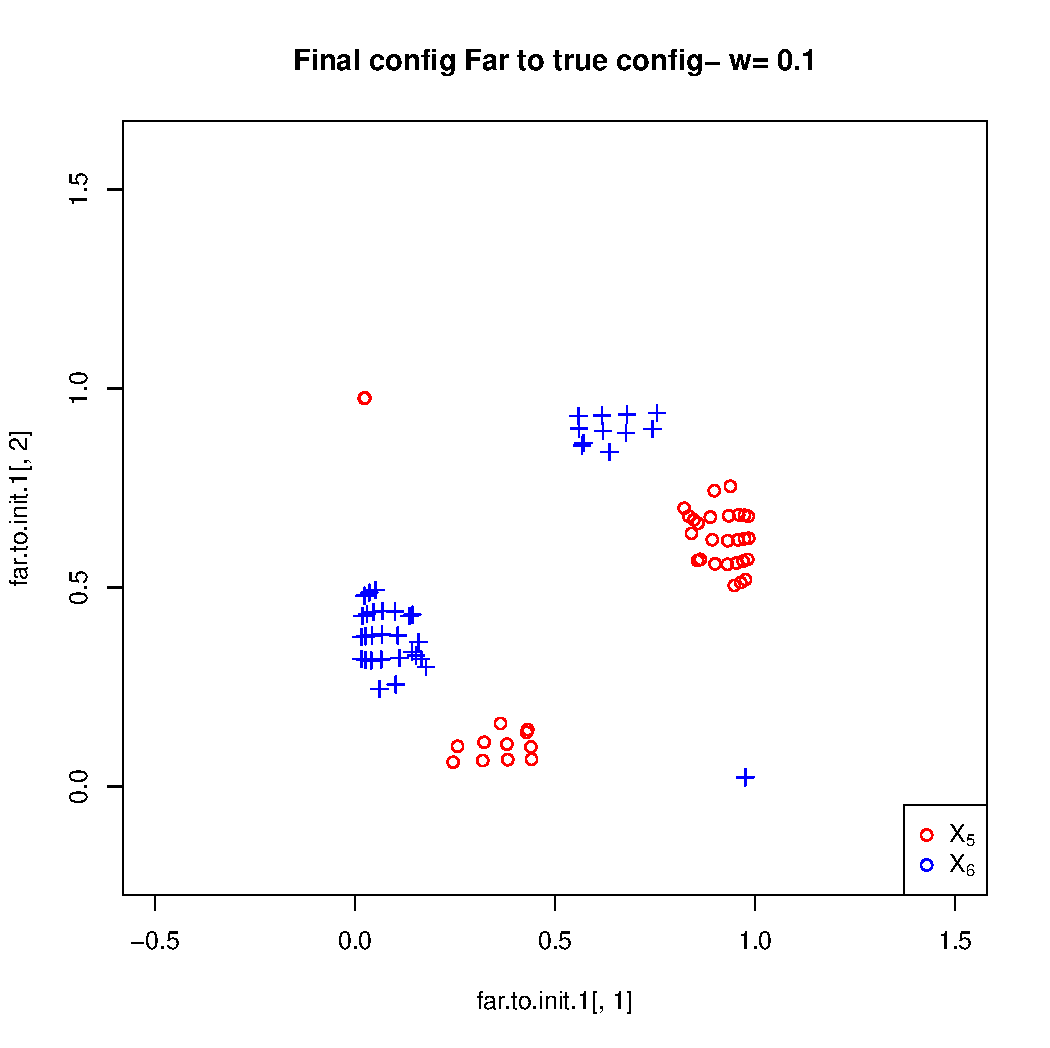
\includegraphics[scale=0.35]{other-min-w-0_1.pdf}

\label{fig:Finalconfig-MultMin-w-0_1_b}
\end{minipage}

\caption{Final configurations for for different $w=0.1$ }
\label{fig:Finalconfig-MultMin-w-0_1}


\end{figure}




\begin{figure}
\begin{minipage}[b]{0.5\linewidth}
\centering
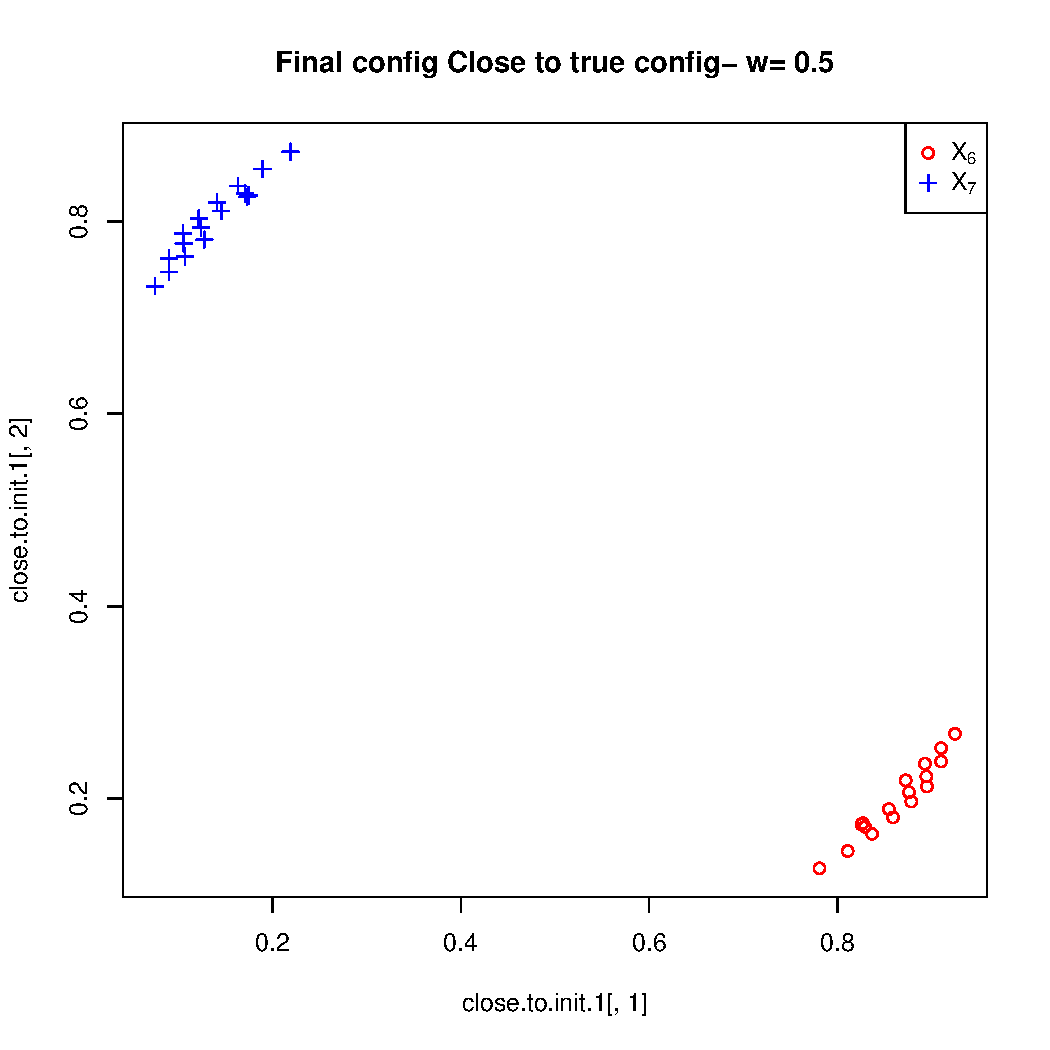
\includegraphics[scale=0.35]{true-min-w0_5}

\label{fig:Finalconfig-MultMin-w-0_5_a}

\end{minipage}
\hspace{0.5cm}
\begin{minipage}[b]{0.5\linewidth}
\centering
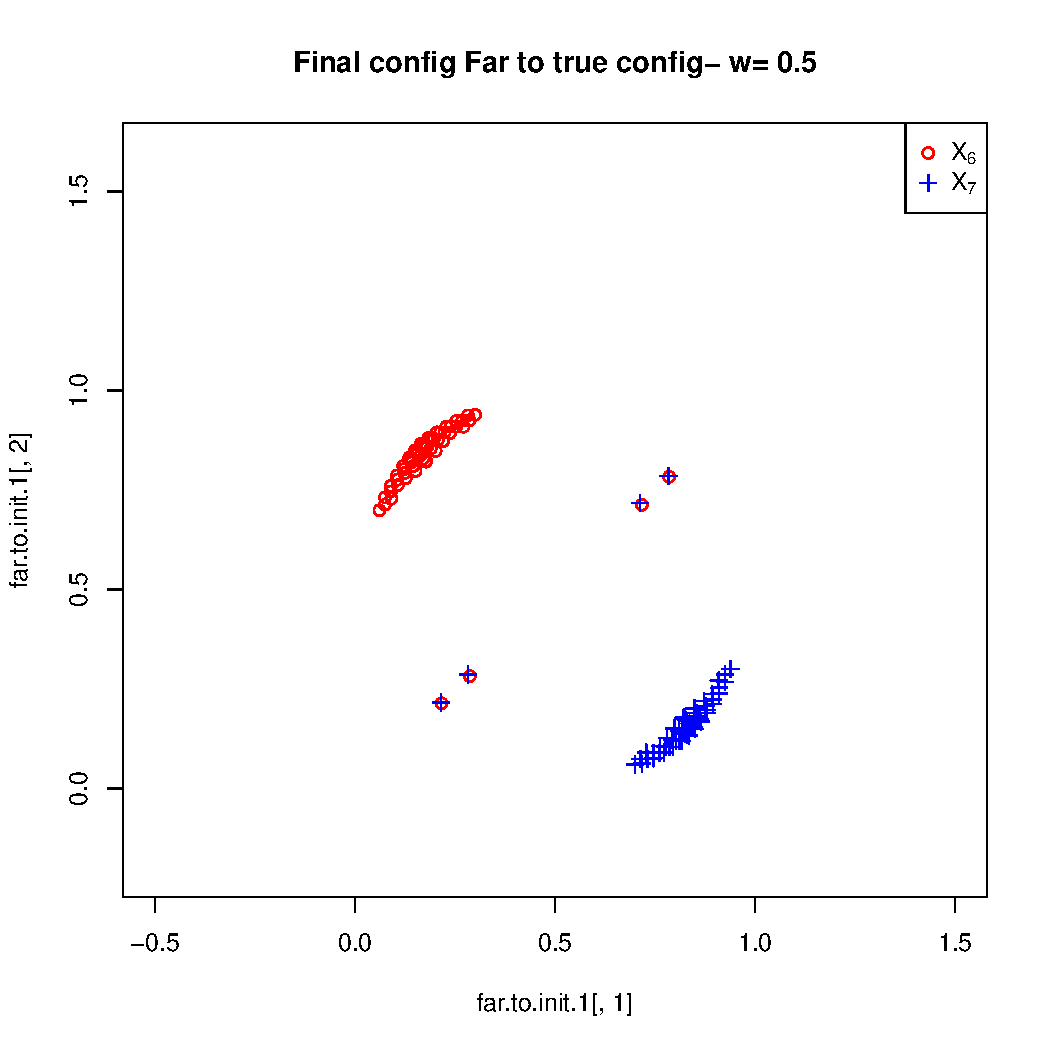
\includegraphics[scale=0.35]{other-min-w0_5.pdf}

\label{fig:Finalconfig-MultMin-w-0_5_b}

\end{minipage}

\caption{Final configurations for for different $w=0.5$ }
\label{fig:Finalconfig-MultMin-w-0_5}

\end{figure}

\begin{figure}
\begin{minipage}[b]{0.5\linewidth}
\centering
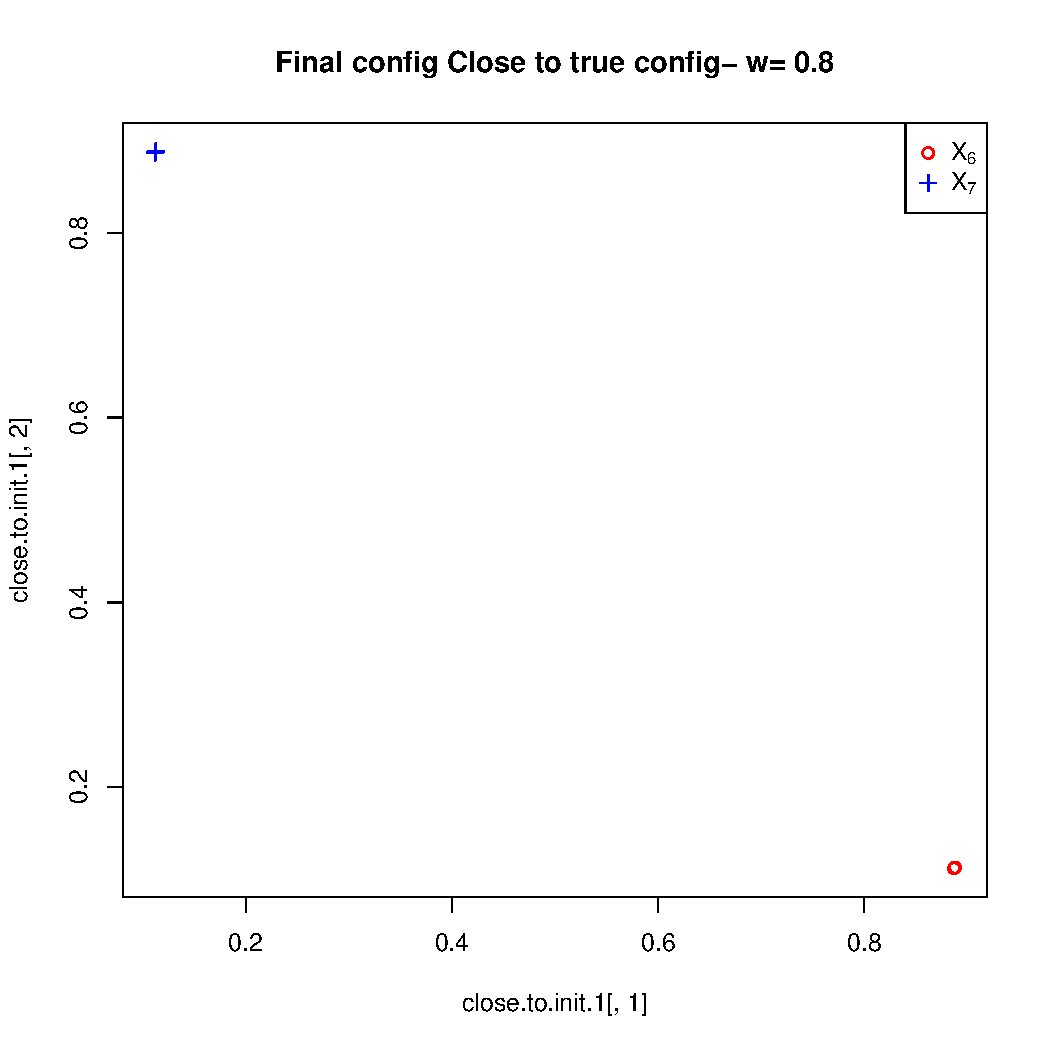
\includegraphics[scale=0.35]{true-min-w0_8.pdf}
\label{fig:Finalconfig-MultMin-w-0_8_a}


\end{minipage}
\hspace{0.5cm}
\begin{minipage}[b]{0.5\linewidth}
\centering
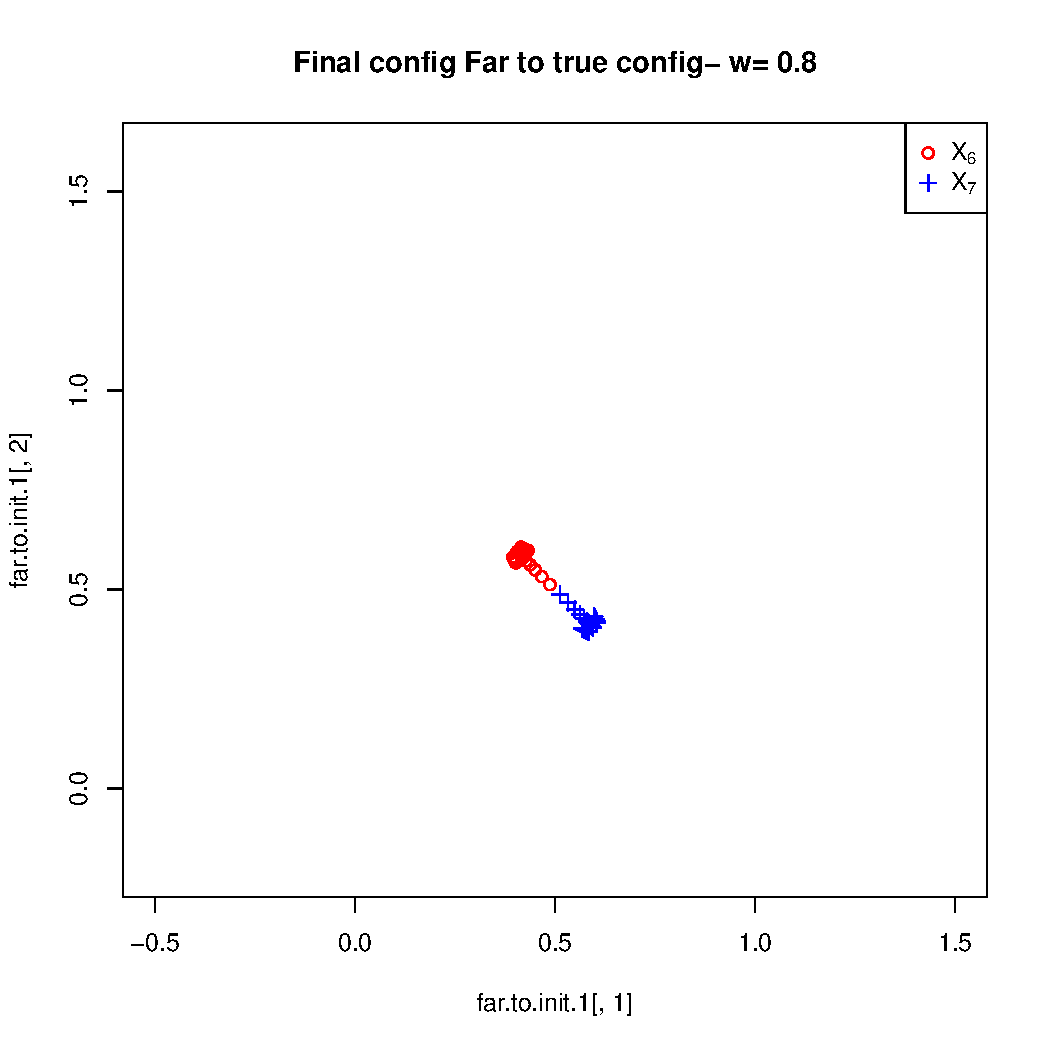
\includegraphics[scale=0.35]{other-min-w0_8.pdf}
\label{fig:Finalconfig-MultMin-w-0_8_a}


\end{minipage}

\caption{Final configurations for for different $w=0.8$ }
\label{fig:Finalconfig-MultMin-w-0_8}

\end{figure}



\begin{figure}
\begin{minipage}[b]{0.5\linewidth}
\centering
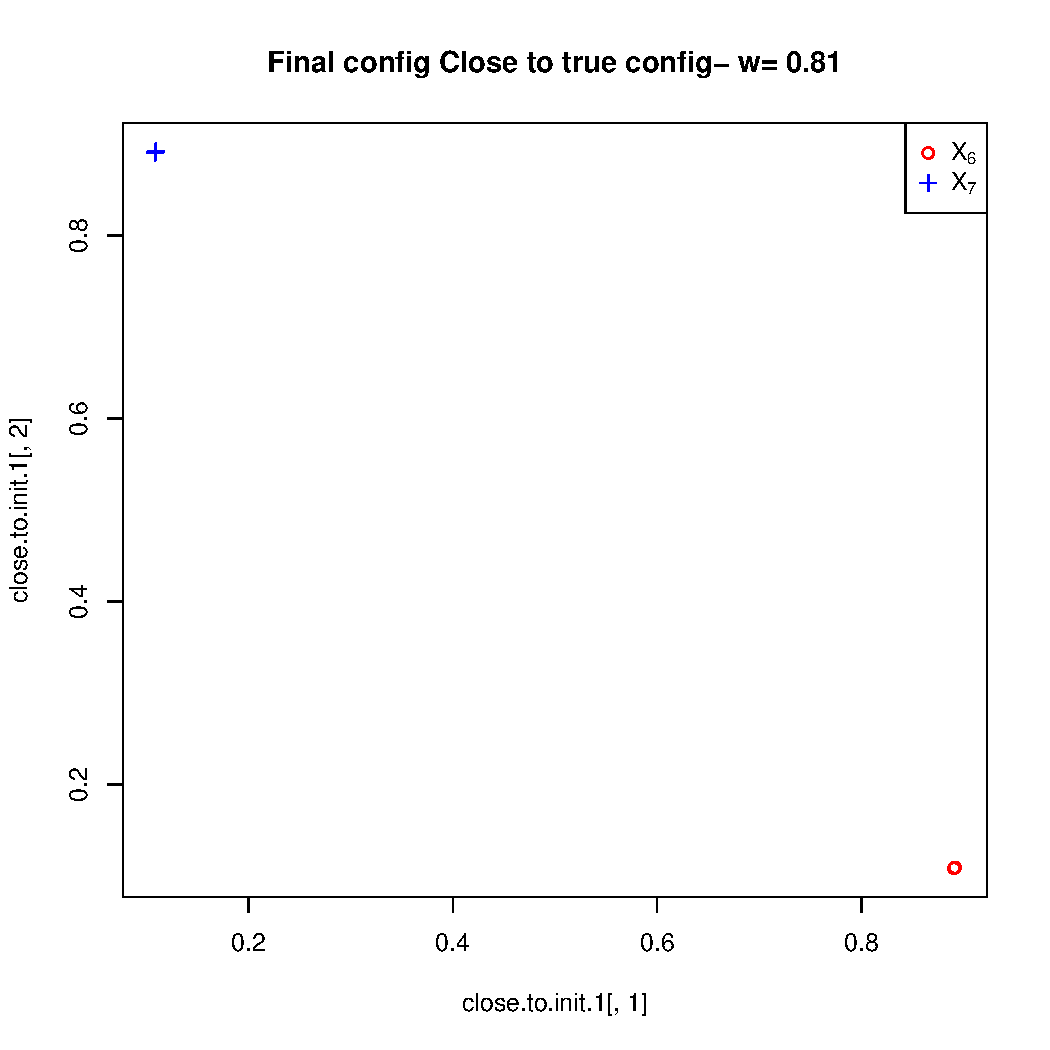
\includegraphics[scale=0.35]{true-min-w0_81.pdf}


\end{minipage}
\hspace{0.5cm}
\begin{minipage}[b]{0.5\linewidth}
\centering
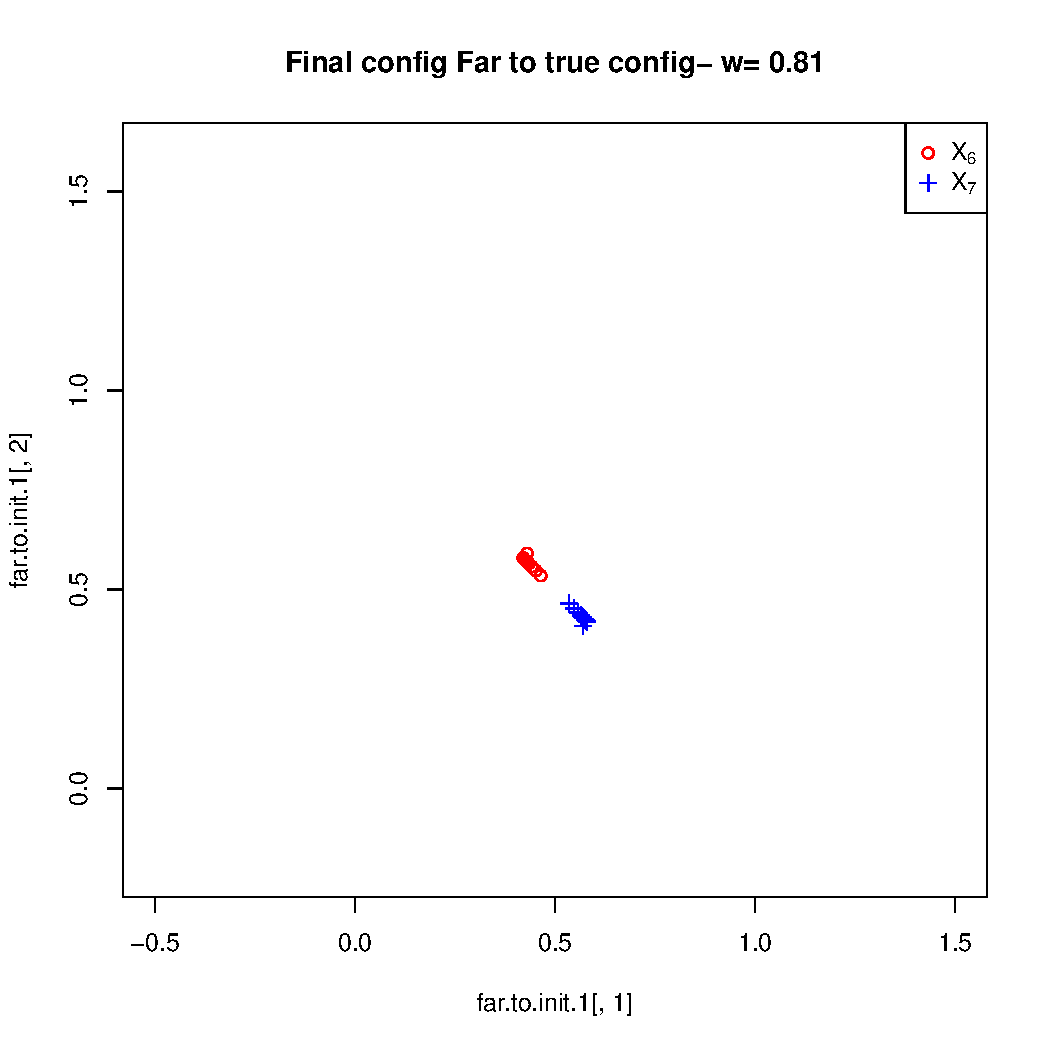
\includegraphics[scale=0.35]{other-min-w0_81.pdf}


\end{minipage}

\caption{Final configurations for for different $w=0.81$ }
\label{fig:Finalconfig-MultMin-w-0_81}

\end{figure}




\begin{figure}
\begin{minipage}[b]{0.5\linewidth}
\centering
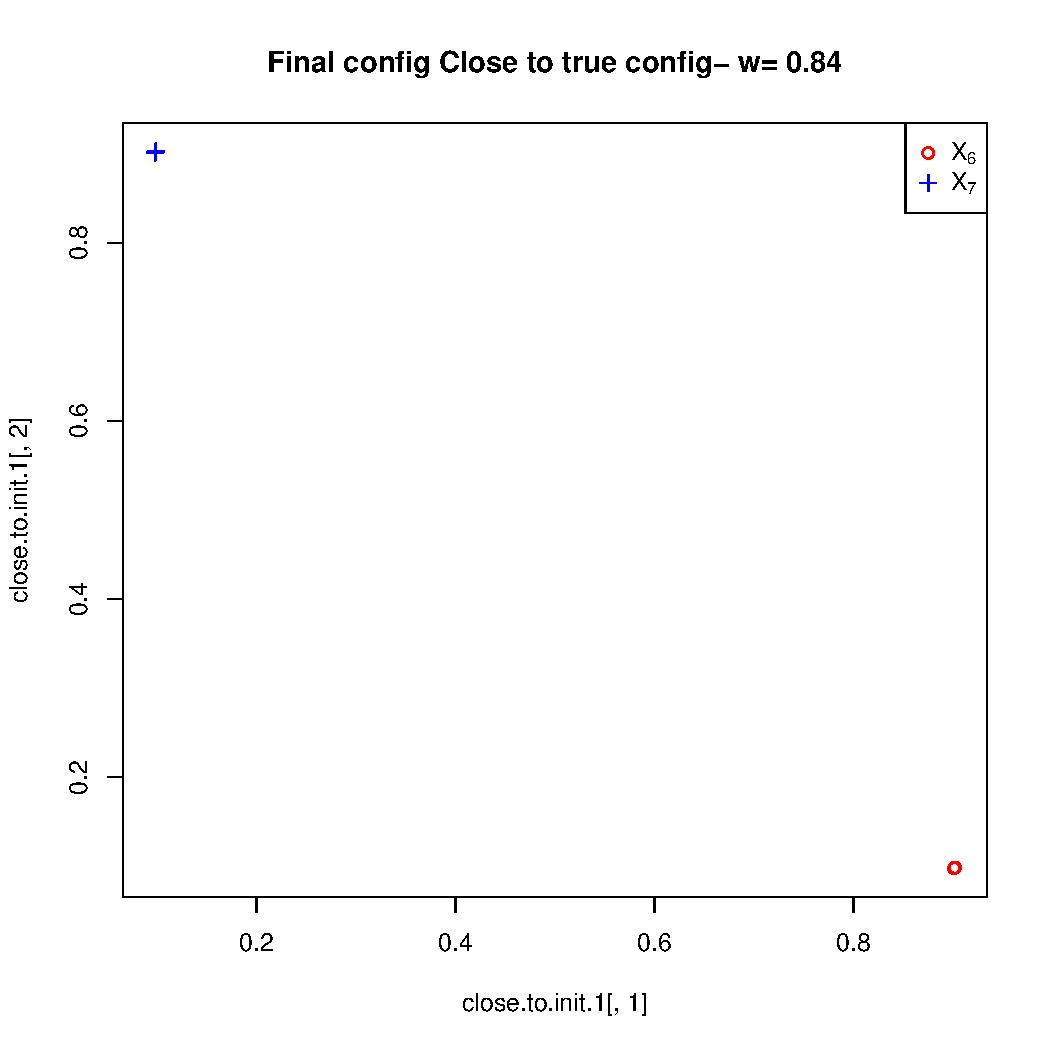
\includegraphics[scale=0.35]{true-min-w0_84.pdf}

\label{fig:figure2-1}
\end{minipage}
\hspace{0.5cm}
\begin{minipage}[b]{0.5\linewidth}
\centering
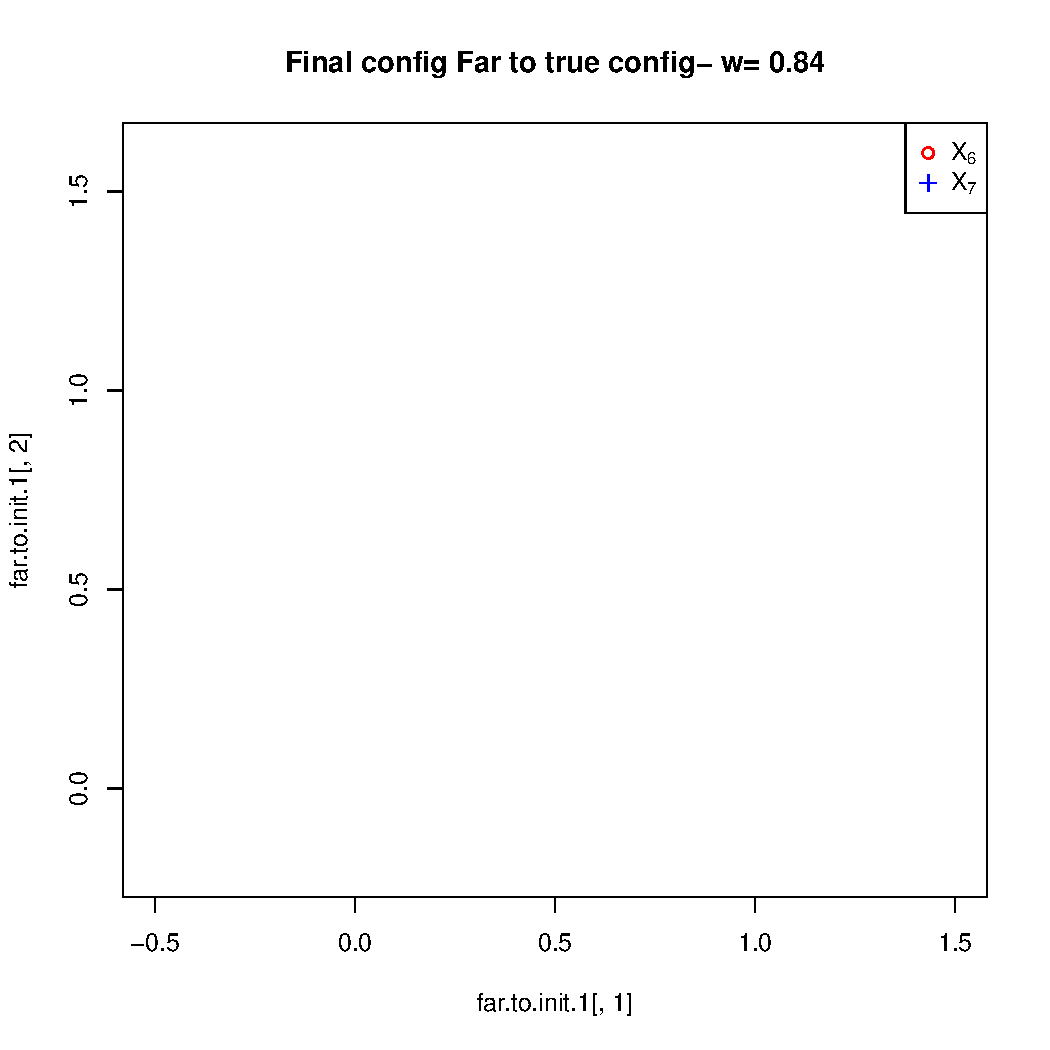
\includegraphics[scale=0.35]{other-min-w0_84.pdf}


\end{minipage}

\caption{Final configurations for for different $w=0.84$ }
\label{fig:Finalconfig-MultMin-w-0_84}

\end{figure}


% latex table generated in R 2.15.1 by xtable 1.7-0 package
% Sat Jan 05 00:54:38 2013

\begin{table}[ht]
\begin{center}

\begin{tabular}{r|rrrrrrrrrrrrrrrrrrrrrrrrrrrrrrrrrrrr}
  \hline
 $w$ & 0.1 & 0.2 & 0.3 & 0.4 & 0.41 & 0.42 & 0.43 & 0.44 & 0.45 & 0.46 & 0.47  \\ 
  \hline
Local min for real config. & 2.80 & 2.51 & 2.22 & 1.92 & 1.89 & 1.86 & 1.83 & 1.80 & 1.77 & 1.74 & 1.71 \\ 
  Alternative local min & 0.39 & 0.76 & 1.10 & 1.40 & 1.43 & 1.46 & 1.48 & 1.51 & 1.53 & 1.56 & 1.58 \\ 
   \hline
\end{tabular}


\begin{tabular}{r|rrrrrrrrrrrrrrrrrrrrrrrrrrrrrrrrrrrr}
  \hline
  $w$ & 0.48 & 0.49 & 0.5 & 0.51 & 0.52 & 0.53 & 0.54 & 0.55 & 0.6 & 0.65 & 0.7 \\ 
  \hline
Local min for real config. &  1.68 & 1.65 & 1.62 & 1.59 & 1.56 & 1.53 & 1.50 & 1.47 & 1.32 & 1.17 & 1.01   \\ 
  Alternative local min &  1.60 & 1.63 & 1.65 & 1.67 & 1.69 & 1.71 & 1.73 & 1.74 & 1.81 & 1.82 & 1.81  \\ 
   \hline
\end{tabular}



\begin{tabular}{r|rrrrrrrrrrrrrrrrrrrrrrrrrrrrrrrrrrrr}
  \hline
 $w$ & 0.75 & 0.76 & 0.77 & 0.78 & 0.79 & 0.8 & 0.81 & 0.82 & 0.83 & 0.84 & 0.85  \\ 
  \hline
Local min for real config. &  0.86 & 0.82 & 0.79 & 0.76 & 0.73 & 0.70 & 0.66 & 0.63 & 0.60 & 0.57 & 0.53  \\ 
  Alternative local min &   1.79 & 1.77 & 1.75 & 1.72 & 1.69 & 1.66 & 1.64 & NA & NA & NA & NA \\ 
   \hline
\end{tabular}

\end{center}

\label{stress-val-table}
\end{table}



\begin{comment}
%old results

\begin{table}[ht]
\begin{center}
\begin{tabular}{rrrrrr}
  \hline
 $w$ value & 0.1 & 0.45 & 0.5 & 0.55 & 0.99 \\ 
  \hline
Local min for real config. & 2.80 & 1.77 & 1.62 & 1.47 & 0.04 \\ 
  Alternative local min & 0.39 & 1.53 & 1.65 & 1.74 & NA \\ 
   \hline
\end{tabular}
\end{center}
\label{stress-val-table}
\end{table}
\end{comment}

Other than such carefully constructed examples, it is  unexpected that slight changes in $w$  will change the ordering of the ``distinct''  local minima according to their stress values.
Therefore,  the argmin among the local minima configurations is independent of $w$. The minimum configuration is then a continuous function of $w$. 
By the continuity of the distance function with respect to configurations, the test statistic is continuous with respect to $w$. One can conclude  that stochastic continuity  is a valid assumption and $\beta(w) $ is a continuous function of $w$. 
%It is possible this is not the global minimum in $\mathbb{R}^d$  

%Does the discontinuity in configurations mean discontinuity  in the $\beta(w)$ function
%It is possible this is not the global minimum in $\mathbb{R}^d$  
 
\begin{comment}

\includegraphics{FidCommPaper-fig-stats-p}



 , so any $w$ value that takes advantage of this situation and captures fidelity will limit the growth of the test statistic under alternative. So such $w$ values that are small enough to preserve fidelity, yet large enough to not lose significantly from commensurability will have increases in power to become $w^*$. 




Consider  an increase in $r$, this will cause the test statistic under null to be stochastically smaller,
 leading to a smaller critical value. So , a increase in priority of fidelity,
  which corresponds to smaller $w$ might lead to the increase in the test statistic under alternative, and therefore an increase in power.\ref{fig-stats-r}  



\includegraphics{FidCommPaper-fig-stats-r}

Consider increases in $c$, which will increase the dissimilarity  both between matched and between unmatched vectors. 



\includegraphics{FidCommPaper-fig-stats-c}




Consider increases in $q$,  the test statistic under both null and alternative is inflated\ref{fig-stats-q}. 


\includegraphics{FidCommPaper-fig-stats-q}
 If commensurability can be preserved in the face of the increase in $q$, the power of the test may be preserved. However a very large increase in $w$ is not guarenteed to increase the preservation of commensurability, since the extra dimensions are noise, trying to   make the differences between coordinates  small in those dimensions will not  help in power, in fact may be disruptive since,
  more fidelity may be lost in the effort to bring the pair of points together.

\end{comment}


\section[Optional table of contents heading]{Dependence of globality of local minima on $w$}
\chapter{Grassmannian Manifold and  Metrics}
\label{sec:Grassmann}
\chaptermark{Optional running chapter heading}

Introduction.

A citation \cite{A}. 
A citation without brackets \citen{B}. 
Multiple citations \cite{A, B, C}.

\section{Grassmannian Manifold}


\section[Optional table of contents heading]{Metrics in Grassmannian Manifold}

\section{Relationship with Commensurability}
\chapter{Application to Vertex Matching in Graphs Problem}
\label{sec:graph-prob}
\chaptermark{Optional running chapter heading}
\chapter{Application to Vertex Matching in Graphs Problem}
\label{sec:graph-prob}
\chaptermark{Optional running chapter heading}

\include{appendix}

%% REFERENCES

% if you use BIBTEX
\bibliographystyle{IEEEtran}
\bibliography{priebe-thesis-JOFC}

\begin{vita}

\begin{wrapfigure}{l}{0pt}

\includegraphics[width=2in,height=2.5in,clip,keepaspectratio]{rjvheadshot}
\end{wrapfigure}



\end{vita}
\end{document}
